\documentclass{beamer}
\usepackage[utf8]{inputenc}
\usepackage{algorithm,algpseudocode}
\usepackage{subcaption}
\usepackage{appendixnumberbeamer}
\usetheme{Madrid}
%\usetheme{Berlin}
\usecolortheme{default}

%------------------------------------------------------------
%This block of code defines the information to appear in the
%Title page
\title[Final Report] %optional
{Final Report of the Guide Study (CS6534)}

\subtitle{Topic: Physical layer key generation for wireless sensor networks}

\author[HUANG Kunlun] % (optional)
{HUANG Kunlun}


\institute[CityU HK] % (optional)
{
  {Supervisor:}

  {Professor XU Weitao}
  \and
  Department of Computer Science\\
  City University of Hong Kong
  
}

\date[Guide Study Presentation] % (optional)
{Guide Study Presentation, December 2023}

\logo{
\includegraphics[height=1cm]{cityulogo}}

%End of title page configuration block
%------------------------------------------------------------



%------------------------------------------------------------
%The next block of commands puts the table of contents at the 
%beginning of each section and highlights the current section:

\AtBeginSection[]
{
  \begin{frame}
    \frametitle{Table of Contents}
    \tableofcontents[currentsection]
  \end{frame}
}
%------------------------------------------------------------


\begin{document}

%The next statement creates the title page.
\frame{\titlepage}


%---------------------------------------------------------
%This block of code is for the table of contents after
%the title page
\begin{frame}
\frametitle{Table of Contents}
\tableofcontents
\end{frame}
%---------------------------------------------------------


\section{Introduction}

%---------------------------------------------------------
%Changing visivility of the text
\begin{frame}
\frametitle{Introduction}
\textbf{Vital:}

Network security is a recent scorching topic and affects everyone's vital interests. PKI-based password management systems such as SSL and TLS are regarded as an excellent way to solve the problem of encrypted communication in computer networks. \pause 
\begin{figure}
  \centering
  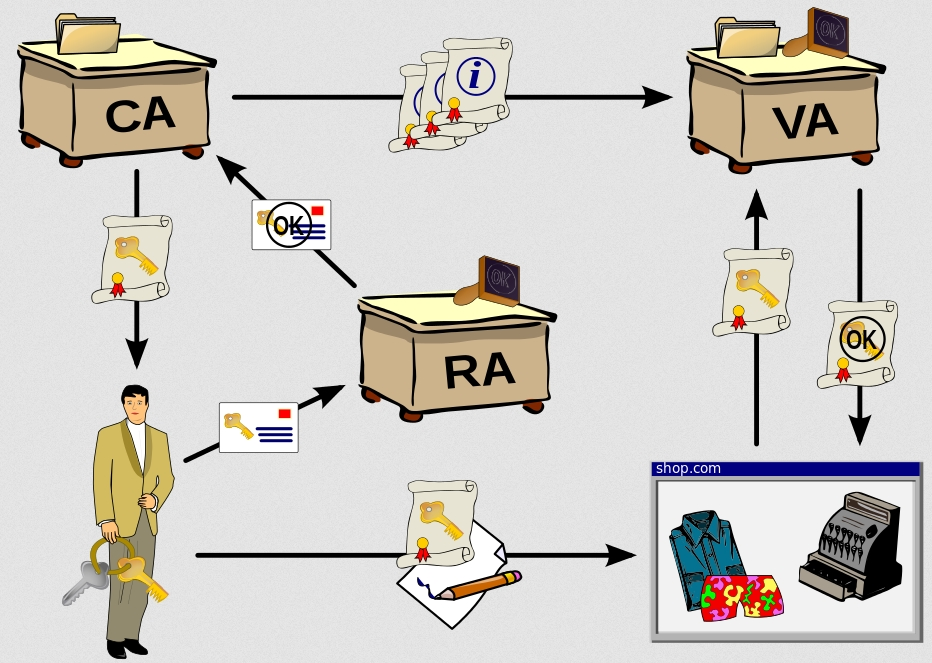
\includegraphics[width=0.4\linewidth]{figures/pkisystem.png}
  \caption{PKI System\cite{wiki:Public_key_infrastructure}}
  \label{fig:pkisystem}
\end{figure}
OK?
\end{frame}

\begin{frame}
\frametitle{Introduction}
\begin{alertblock}{Not Suitable}
  However, in the field of the Internet of Things(IoT), due to issues such as node computing performance and the difficulties in key management in large amount of nodes, PKI systems are \textbf{not suitable} in it. 

\end{alertblock}
\vspace{0.05in}
\end{frame}

\begin{frame}
  \frametitle{Introduction}
\textbf{Rapid Growing of IoT Market:}

According to Gartner\cite{gartnerresearchiot}, there will be over 43 billion IoT devices connected to the internet by 2023, and the IoT market size will reach US\$1.4 trillion. The rapid development of the IoT is mainly due to the following trends. Also, the MIIT suggests that the IoT is a future development trend that will have a profound impact on all industries\cite{iot13th5yr}. 

\begin{figure}
  \centering
  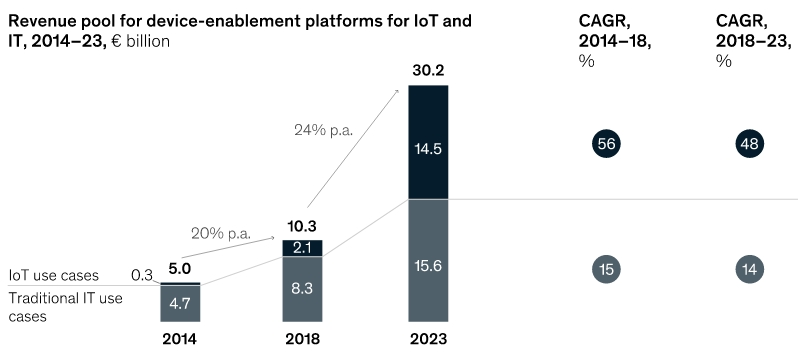
\includegraphics[width=0.7\linewidth]{figures/iotgrowing.png}
  \caption{IoT Growing\cite{Dahlqvist_Patel_Rajko_Shulman_2019}}
  \label{fig:iotgrowing}
\end{figure}

\end{frame}

%---------------------------------------------------------


%---------------------------------------------------------
\begin{frame}
\frametitle{Introduction}

To address this problem, \textbf{Physical layer key generation(PLKG)} have been proposed. Which is a technique for generating cryptographic keys from the physical characteristics of a wireless communication channel. This can be done by exploiting the unique features of the channel, such as its fading characteristics, noise properties, and path loss. \pause
\begin{block}{Attractive}
  PLKG particularly attractive for wireless sensor networks (WSNs) because it does not require any prior shared information between the nodes, and it can be implemented with relatively low computational overhead.
\end{block}

\end{frame}

\begin{frame}
\frametitle{Introduction}
  
Physical layer key generation has recently been a research hotspot in academia and industry\cite{7120014}, focuses only on traditional wireless  technologies such as Wi-Fi, ZigBee, and 5G Radio Access Network. 

In the area of Low-Power Wide-Area Networks (LPWAN)\cite{iotfactorylpwan}, the \textbf{long communication distance, low power consumption, and low trans rate} bring new research challenges to physical layer key generation.
  
  \begin{figure}
    \centering
    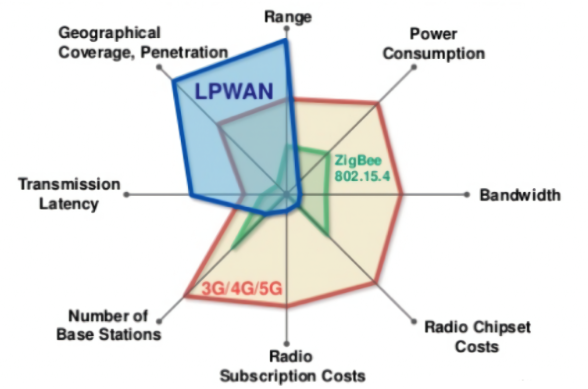
\includegraphics[width=0.42\linewidth]{../figures/fig1-1.png}
    \caption{LPWAN vs. Other wireless communication technologies\cite{iotfactorylpwan}}
    \label{fig:1-1}
  \end{figure}
\end{frame}


%---------------------------------------------------------
% Example
%---------------------------------------------------------

\section{Related Work}

%---------------------------------------------------------
\begin{frame}
\frametitle{Related Work - Physical Layer Key Generation}
Generally, physical layer key generation applies the following five steps to generate a key: channel probing, randomness extraction, quantization, information reconciliation, and privacy amplification\cite{7120014}.
\begin{figure}
  \centering
  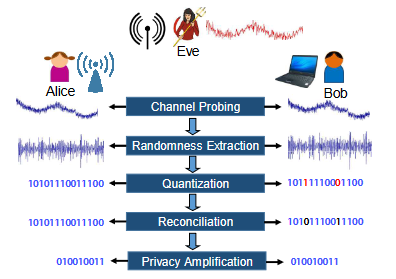
\includegraphics[width=0.6\linewidth]{../figures/fig2-1.png}
  \caption{Physical Layer key Generation Model\cite{7120014}}
  \label{fig:phykegen}
\end{figure}

\end{frame}

\begin{frame}
  \frametitle{Related Work - LoRa}
  LoRa, a widely used LPWAN communication technology, is a physical layer modulation method defined by Semtech Corporation.
  LoRa embraces the Chirp Spread Spectrum (CSS) modulation mechanism, offering both anti-interference capabilities and the ability for long-range communication.
  \begin{figure}
    \centering
    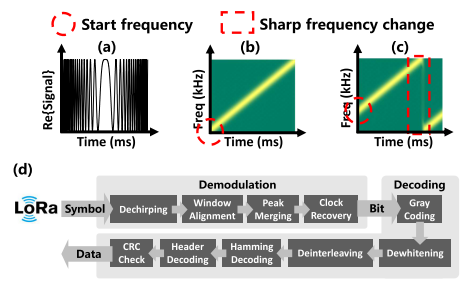
\includegraphics[width=0.6\linewidth]{../figures/fig2-2.png}
    \caption{LoRa PHY\cite{10.1145/3546869}}
    \label{fig:2-2}
  \end{figure}
  
\end{frame}
%---------------------------------------------------------
\begin{frame}
  \frametitle{Related Work - Existing Solutions}
  \begin{itemize}
    \item CFR-Based Physical Layer Key Generation
    \item RSSI-Based Physical Layer Key Generation
    \item Chaos-based Physical Layer Key Generation
    \item Deep-Learning-Based Physical Layer Key Generation
    \item Quantum-Based Physical Layer Key Distribution
\end{itemize}
\end{frame}


\begin{frame}
  \frametitle{Related Work - Existing Solutions}
  \begin{itemize}
    \item CFR-Based Physical Layer Key Generation\cite{7054386}\cite{10158732}
    
    When receiving \(I_{MS}\), both BS and MS construct a CFR estimate vector at the agreed subcarrier index set \(I_{MS}\) as:
\begin{equation} 
  \hat{H}_{U}(I_{MS})   = \left [ \hat{H}_{U}(f_{(1)})\hat{H}_{U}(f_{(2)}) ...\hat{H}_{U}(f_{1(T_{b})}) \right ], where\ u\in \left \{ BS, MS  \right \}   
\end{equation} 
and then generate the secret key by:
\begin{equation} 
  K_{U}  = \left [ K_{U}({(1)})K_{U}{(2)} ...K_{U}({2T_{b}}) \right ]
\end{equation} 
The CFR is an unique characteristic of the LoRa channel that depends on the distance, orientation, and other environmental factors.

\end{itemize}
\end{frame}

\begin{frame}
  \frametitle{Related Work - Existing Solutions}
  \begin{itemize}
    \item RSSI-Based Physical Layer Key Generation\cite{10.1145/1614320.1614356}\cite{8580375}
    
    Using the received signal strength indicators (RSSI) employed a number of signal processing techniques to improve key generation rate significantly and proposed a novel compressive sensing-based reconciliation framework to reduce the mismatch rate\cite{8580375}. 
\begin{equation} y = y_{\mathrm{ Bob}}-y_{\mathrm{ Alice}}= A \left ({K_{\mathrm{ Bob}}-K_{\mathrm{ Alice}}}\right) + e= A x +e \end{equation} 
\begin{equation} \mathop {\mathrm {arg\,min}} _{x} \| x \|_{1} \quad \text {subject to}~ ~\left \|{y - Ax}\right \|_{2} < \epsilon.\end{equation} 
\begin{equation}K_{\mathrm{ Alice}}^{'} = K_{\mathrm{ Alice}} \oplus x\end{equation} 
\end{itemize}
\end{frame}

\begin{frame}
  \frametitle{Related Work - Existing Solutions}
  \begin{itemize}
    \item Chaos-based Physical Layer Key Generation\cite{https://doi.org/10.1049/iet-opt.2018.5072}
    
    The chaotic behavior of the wireless channel can be exploited to generate a random bit sequence that is used as a secret key shared only between the communicating devices. When including the position-sensitive and real-valued channel state information of the VLC channel. 
    \begin{equation}{\widehat {\mathbf{s}}_k} = \arg \mathop {\min }\limits_{{\mathbf{s}}_k^{(i)} \in {\mathbf{S}}} {\left\| {{{\mathbf{r}}^{(k)}} - {h_k}{\mathbf{s}}_k^{(i)}} \right\|^2};k = 1, \ldots ,K\end{equation}
    where
    \begin{equation}{{\mathbf{r}}^{(k)}} = \begin{cases} {\mathbf{r}}&{;{\text{ for }}k = 1} \\ {{{\mathbf{r}}^{(k - 1)}} - {h_{k - 1}}{{\widehat {\mathbf{s}}}_{k - 1}}}&{;{\text{ for }}k = 2, \ldots ,K.} \end{cases}\end{equation}
    then, the output of the \(k^{th}\) stage is demodulated as \({{\hat{\mathbf b}}_k} = \left[ {\begin{array}{lll} {{{\hat b}_{k,1}}}& \ldots &{{{\hat b}_{k,U}}} \end{array}} \right]\).
\end{itemize}
\end{frame}

\begin{frame}
  \frametitle{Related Work - Existing Solutions}
  \begin{itemize}
    \item Deep-Learning-Based Physical Layer Key Generation\cite{9526766}
    
    Deep learning or machine learning algorithms can be used to analyze the wireless channel characteristics and identify patterns that can be used to generate a secret key.
    a Deep-Learning-Based Physical-Layer Secret Key Generation for FDD Systems using the adaptive moment estimation (ADAM) algorithm with the following loss function\cite{9526766}. 
\begin{equation} {\mathrm{ Loss}}_{\mathbb {D}}\left ({\boldsymbol {\Omega }}\right) = {\mathrm{ MSE}}\left ({\widehat {\mathbf {x}}_{2}, \mathbf {x}_{2}}\right)=\frac {1}{VN_{\mathbf {x}}}\sum _{v=0}^{V-1}\left \|{\widehat {\mathbf {x}}_{2}^{\left ({v}\right)} -\mathbf {x}_{2}^{\left ({v}\right)}}\right \|_{2}^{2}\end{equation} 

\end{itemize}
\end{frame}

\begin{frame}
  \frametitle{Related Work - Existing Solutions}
  \begin{itemize}
    \item Quantum-Based Physical Layer Key Distribution
    
    Using quantum mechanics principles for physical layer key distribution is also a promising approach for wireless networks. Quantum mechanics principles can be applied to generate truly random keys using the quantum states of particles. 
    \begin{figure}
      \centering
      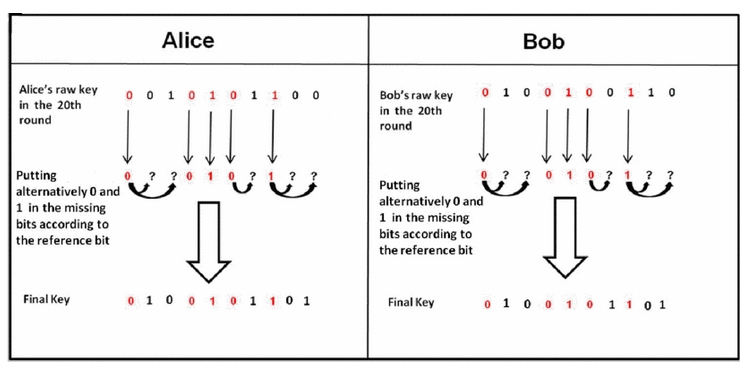
\includegraphics[width=0.6\linewidth]{figures/quantum.png}
      \caption{Quantum Sifted key\cite{10.1145/3546869}}
      \label{fig:quantum}
    \end{figure}
\end{itemize}
\end{frame}

\begin{frame}
  \frametitle{Related Work - Existing Solutions}

  \begin{block}{IoT WSNs Factors}
    CPU and memory specifications limitation, is designed for Low-Power and Battery-Operated
  \end{block}
  
  \begin{itemize}
    \item CFR-Based Physical Layer Key Generation
    \item \alert{RSSI-Based Physical Layer Key Generation}
    \item Chaos-based Physical Layer Key Generation
    \item Deep-Learning-Based Physical Layer Key Generation
    \item Quantum-Based Physical Layer Key Distribution
\end{itemize}
\end{frame}

%---------------------------------------------------------

\section{Project Outline and Methodology}

%---------------------------------------------------------
\begin{frame}
  \frametitle{Project Outline and Methodology}
  \begin{itemize}
    \item The implementation of LoRa nodes’ communication, such as signal sending and receiving, coding and decoding
    \item The extraction and analysis of the physical layer information between the communication process
    \item The implementation of the LoRa key generation and the test on it
    \end{itemize}
\end{frame}

\begin{frame}
  \frametitle{LoRa Physical Layer Emulation and Analyst}
  The LoRaPHY KIT is for LoRa Physical Protocol emulation\cite{10.1145/3546869}. Through this KIT, the payload of LoRa can be simulated, especially, and the encryption information can be analyzed and visualized before and after.
\begin{figure}
  \centering
  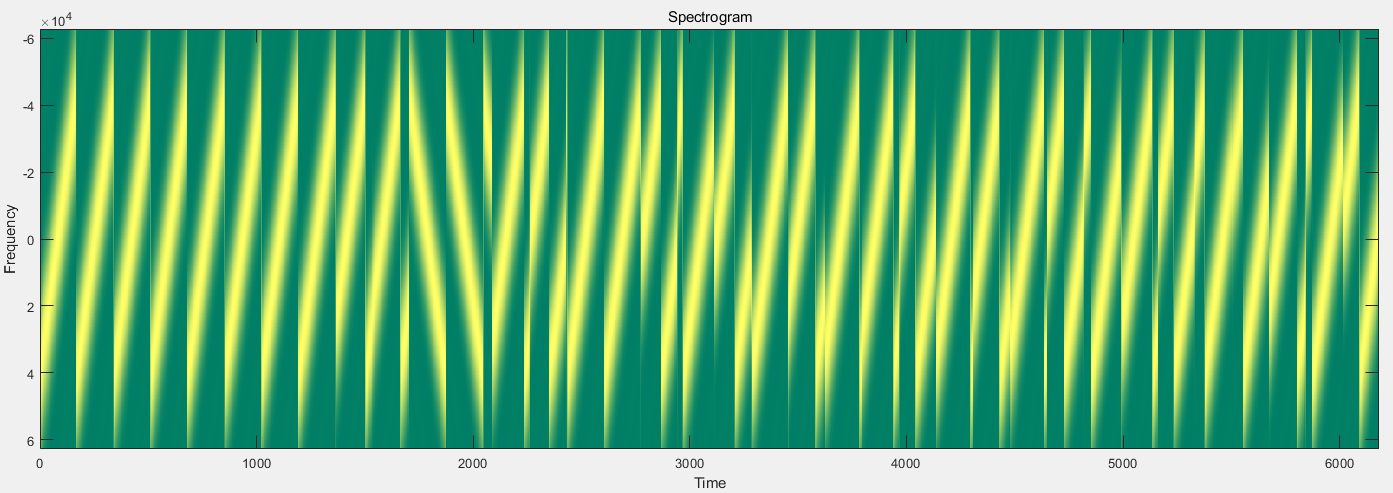
\includegraphics[width=0.8\linewidth]{../figures/fig3-1.png}
  \caption{A emulated LoRa physical layer payload of ‘[78 22 43 44 12]’}
  \label{fig:3-1}
\end{figure}
\end{frame}

\begin{frame}
  \frametitle{Arduino Shield featuring LoRa technology}
  LoRa commonly employs the SX127x chipset manufactured by Semtech, depicted in Figure. An Arduino Shield, incorporating LoRa technology and the computing and controlling.
  \begin{figure}
    \centering
    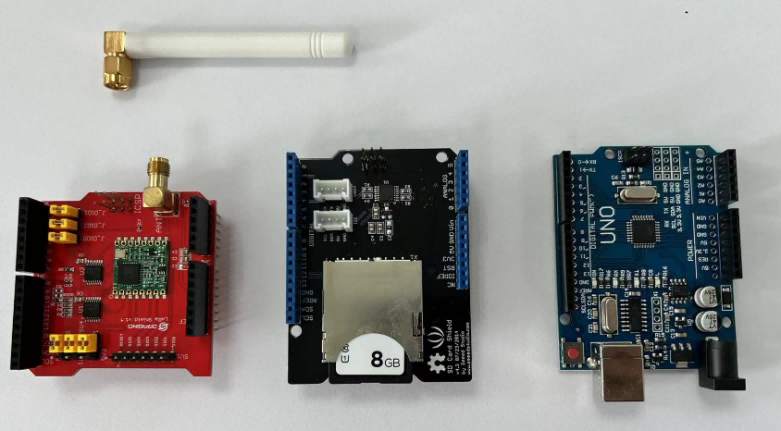
\includegraphics[width=0.6\linewidth]{../figures/fig3-3.png}
    \caption{The SX127x and Arduino’s UNO Programmable Board}
    \label{fig:3-3}
  \end{figure}
\end{frame}

\begin{frame}
  \frametitle{Deep-in-Building and Outdoor Test}
  The outdoor test regimen for LoRa communication entails a meticulous assessment of the system's performance attributes in open-air or outdoor settings, characterized by the absence of indoor obstructions.Remote areas like the wilderness or deep in the mountains
  \begin{figure}
    \centering
    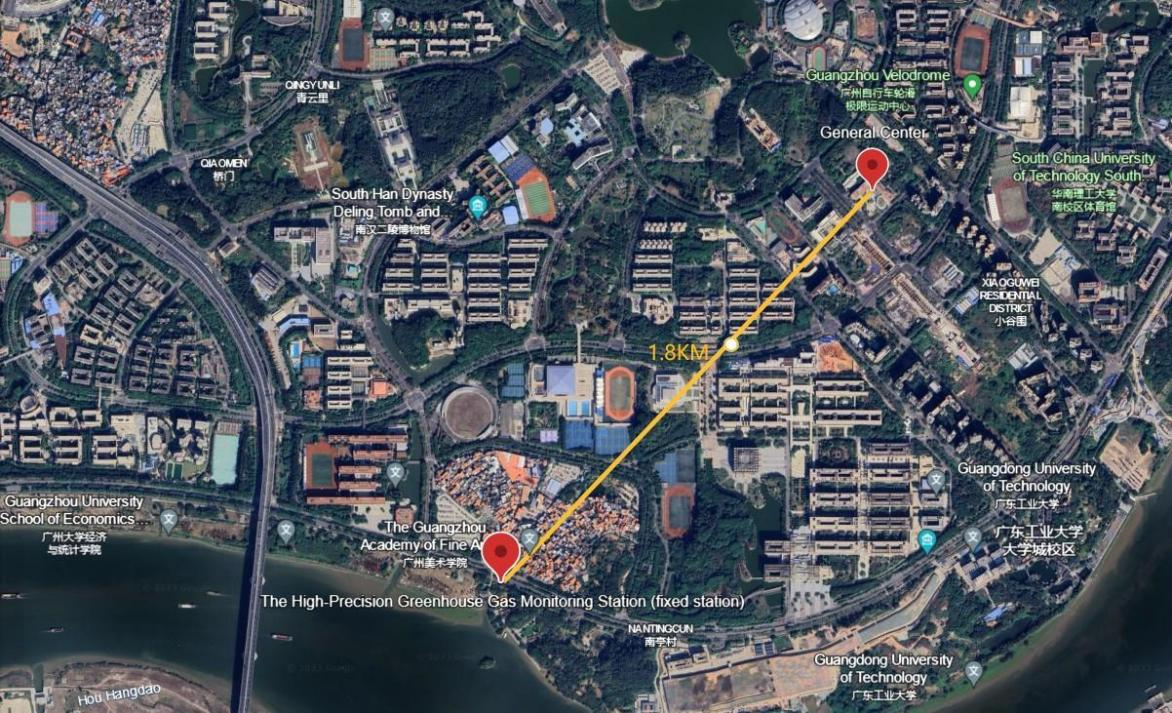
\includegraphics[width=0.55\linewidth]{../figures/fig3-4.png}
    \caption{Outdoor test between an fixed High-Precision Greenhouse Gas Monitoring Station and the Complex Building (1.8km)}
    \label{fig:3-4}
  \end{figure}
\end{frame}

\begin{frame}
  \frametitle{Deep-in-Building and Outdoor Test}
  The principal objective of the deep-in-building test for LoRa communication is to scrutinize the signal propagation characteristics within the intricate confines of interior structures, encompassing walls, floors, and architectural elements.
  \begin{figure}
    \centering
    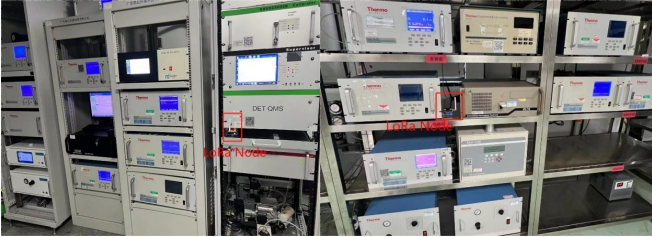
\includegraphics[width=0.8\linewidth]{../figures/fig3-5.png}
    \caption{Deep-In-Building Test at Complex Building}
    \label{fig:3-5}
  \end{figure}
\end{frame}

\begin{frame}
  \frametitle{Data Extraction and Analyst}

  In particular, the analysis of feature data from the signals. Through the analysis of this data, we can understand the characteristics of LoRa signal features in different scenarios and under different electromagnetic background interferences.
  \begin{itemize}
    \item Sampling RSSI
    \item Preprocess the data
    \item Data Extraction and Analyst
    \item Physical Key Generation
  \end{itemize}
\end{frame}

%---------------------------------------------------------

\section{System Modeling and Implementation}

%---------------------------------------------------------
%Example of the \pause command
\begin{frame}
  \frametitle{Communication Architecture}
  \begin{columns}

    \column{0.4\textwidth}
    The architecture mainly describes Alice and Bob as two LoRa nodes that need to generate the same communication key. It starts with one of them initiating the key generation communication (a random LoRa message with a sequence number). When the other party (Bob) receives the request, it immediately replies with a message with a sequence number.
    
    \column{0.6\textwidth}
    \begin{figure}
      \centering
      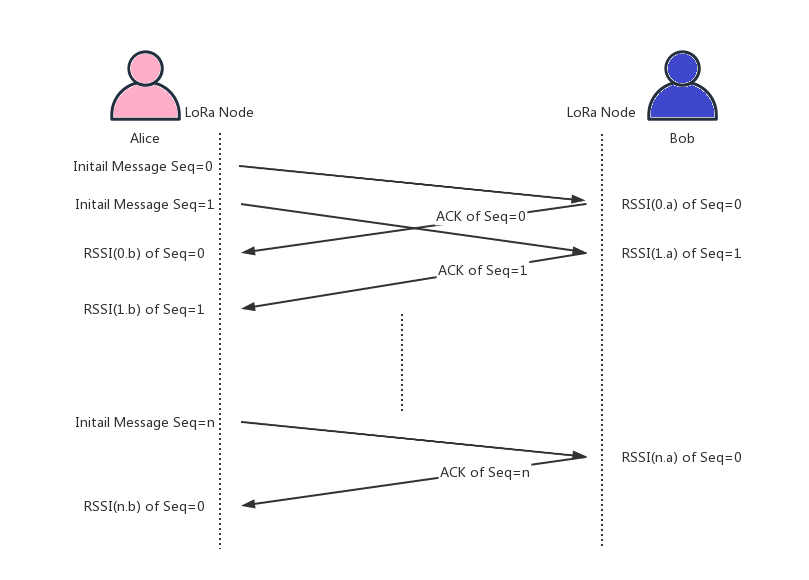
\includegraphics[width=1\linewidth]{../figures/fig4-1.png}
      \caption{Communication Architecture}
      \label{fig:4-1}
    \end{figure}
    \end{columns}
\end{frame}

\begin{frame}
  \frametitle{LoRa End Nodes Modeling and Algorithm}

  As mentioned in the previous text, LoRa nodes are half-duplex devices. In order to implement the mentioned functional model, a specific algorithm is required to enable LoRa nodes to both listen to messages and transmit messages after receiving information.
  \begin{itemize}
    \item Algorithm for Alice
    \item Algorithm for Bob
    \item onReceive Algorithm for Alice
    \item onReceive Algorithm for Bob
    \item Algorithm for sendMessage
  \end{itemize}
\end{frame}

\begin{frame}
  \frametitle{LoRa End Nodes Modeling and Algorithm}
    \begin{algorithm}[H]
      \caption{Algorithm for Alice}\label{alg:Alice}
      \begin{algorithmic}
      \State Initialize variables:
          \State $lastSendTime \gets 0$
          \State $interval \gets$ user-defined interval
          
          \Function{loop}{}
              \If{$\text{millis()} - \text{lastSendTime} > \text{interval}$}
                  \State $message \gets \text{``SEQ"} \gets n$
                  \State \Call{sendMessage}{$message$}
                  \State \textbf{print} ``Sending" $+$ $message$
                  \State $lastSendTime \gets \text{millis()}$
                  \State $interval \gets \text{random}(2000) + 1000$ \Comment{2-3 seconds}
              \EndIf
              \State \textbf{parse for a packet, and call} \Call{onReceive}{\text{parsePacket()}}
          \EndFunction
      \end{algorithmic}
    \end{algorithm}
\end{frame}

\begin{frame}
  \frametitle{LoRa End Nodes Modeling and Algorithm}
  \begin{algorithm}[H]
    \caption{onReceive Algorithm for Alice}\label{alg:onReceive}
    \begin{algorithmic}
        \Function{onReceive}{$\text{packetSize}$}

            \State Perform packet checking

            \State \vdots 

            \If{$recipient \neq \text{localAddress} \land recipient \neq 0xFF$}
                \State \textbf{print} ``This message is not for me."
                \State \textbf{return}
            \EndIf
            \State \Comment{Print message details for this device or broadcast:}
            \State \textbf{print} $message$
        \EndFunction
    \end{algorithmic}
\end{algorithm}
\end{frame}

\begin{frame}
  \frametitle{LoRa End Nodes Modeling and Algorithm}
  \begin{algorithm}[H]
    \caption{Algorithm for Bob}\label{alg:Bob}
    \begin{algorithmic}
    \State Initialize variables
        
        \Function{loop}{}
            \State \textbf{parse for a packet, and call} \Call{onReceive}{\text{parsePacket()}}
        \EndFunction
    \end{algorithmic}
  \end{algorithm}
  \begin{algorithm}[H]
    \caption{onReceive Algorithm for Bob}\label{alg:BobonReceive}
    \begin{algorithmic}
        \Function{onReceive}{$\text{packetSize}$}
            \State perform onReceive Algorithm for Alice
            \State $outgoing \gets incoming.SEQ$
            \State \textbf{print} $sendMessage(outgoing)$
        \EndFunction
    \end{algorithmic}
  \end{algorithm}
\end{frame}

\begin{frame}
  \frametitle{Physical Layer Key Generation Modeling and Algorithm}
  After the LoRa end node setup, we can process the physical layer key generation by the following steps:
  \begin{itemize}
    \item Sampling, Proprcessing
    \item RSSI-Based Key Generation Algorithm
    \item Multilevel Quantization
    \item Reconciliation
    \item Privacy Amplification
  \end{itemize}
\end{frame}

\begin{frame}
  \frametitle{Physical Layer Key Generation Modeling and Algorithm}
  Alice and Bob exchange a number of probe and response packets to sample the RSSI channel by the mentioned LoRa End Nodes Modeling and Algorithm. Alice and Bob apply outlier detection and Savitzky–Golay filter.
  \begin{columns}
  \column{0.5\textwidth}
  \begin{equation}
    \begin{bmatrix}
      S_0 & S_1 & \ldots & S_{2k} \\
      S_1 & S_2 & \ldots & S_{2k+1} \\
      \vdots & \vdots & \ddots & \vdots \\
      S_{2k} & S_{2k+1} & \ldots & S_{4k}
    \end{bmatrix}
    \begin{bmatrix}
      c_{-k} \\
      c_{-(k-1)} \\
      \vdots \\
      c_k
    \end{bmatrix}
    =
    \begin{bmatrix}
      0 \\
      0 \\
      \vdots \\
      1
    \end{bmatrix}
    \end{equation}
    \column{0.5\textwidth}

    \begin{figure}
      \centering
      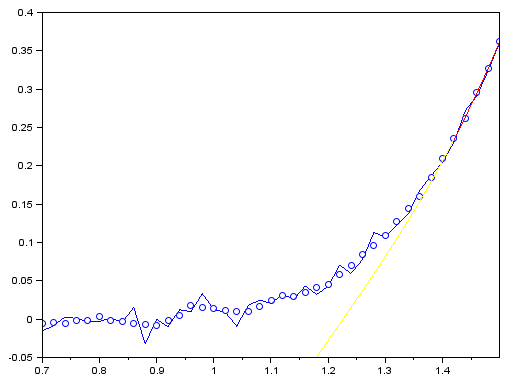
\includegraphics[width=0.6\linewidth]{../figures/fig3-6.png}
      \caption{Savitzky-Golay filter}
      \label{fig:3-6}
    \end{figure}
  \end{columns}
  \(c_j\) are the Savitzky–Golay coefficients where \(S_j = \sum_{i=1}^{n} x_i^j\). The solution to this system provides the coefficients \(c_j\) for the convolution operation.
\end{frame}

\begin{frame}
  \frametitle{LoRa End Nodes Modeling and Algorithm}
  \begin{algorithm}[H]
    \caption{RSSI-Based Key Generation Algorithm}\label{alg:keygeneration}
    \begin{algorithmic}
    
    \Require $X_A$ and $X_B$ :  the original sample RSSI list
    
    \State Initialize variables
    
    \State $X_A'$, $X_B'$ $\gets$ Savitzky–Golay filter($X_A$, $X_B$)
    \Repeat
        \State $K_A'$ $\gets$ Quantization($X_A'$)
        \State $K_B'$ $\gets$ Quantization($X_B'$)
    \Until{$K_A'' \gets Reconciliation(K_A') = K_B'$}
    
    \State $K_{Share} \gets$ Privacy\_Amplification($K_A''$, $K_B'$)
    
    \State \Return $K_{Share}$ \Comment{Secret Key for Alice and Bob}
    
    \end{algorithmic}
  \end{algorithm}
\end{frame}

\begin{frame}
  \frametitle{LoRa End Nodes Modeling and Algorithm}
  \begin{algorithm}[H]
    \caption{Multilevel Quantization}\label{alg:Quantization}
    \begin{algorithmic}
    \Function{Quantization}{$\text{sampleArray}, \text{numBitsPerSample}, \text{alpha}$}
        \State $Variables\ Initailzation$
    
        \For{$i \gets 1$ \textbf{to} $\text{sampleArrayLength}$}
            \For{$j \gets 1$ \textbf{to} $M$}
                \State \vdots \Comment{Listed in Report and source code}
            \EndFor
        \EndFor
        \State $Variables\ Updating$
    
        \For{$i \gets 1$ \textbf{to} $\text{decimalValArrayLen}$}
            \State $\text{bitString}.\text{extend}(\text{format}(\text{decimalValArray}[i], \text{f}'0\{\text{numBitsPerSample}\}b'))$
        \EndFor
    
        \State \Return $\text{bitString}$
    \EndFunction
    \end{algorithmic}
  \end{algorithm}
\end{frame}

\begin{frame}
  \frametitle{LoRa End Nodes Modeling and Algorithm}
  Alice use a CS-based reconciliation method to correct the bit mismatches.
  \begin{algorithm}[H]
    \caption{Reconciliation Algorithm}\label{alg:Reconciliation}
    \begin{algorithmic}
    \Function{Reconciliation}{$A, y$}
        \State $Variables\ Initailzation$
    
        \For{$\text{iter\_idx} \gets 1$ \textbf{to} $\text{iter\_times}$}
            \State $\text{c} \gets A^T \cdot (y - A \cdot x)$
            \State \vdots \Comment{Listed in Report and source code}
            \State $x[\text{act\_set}] \gets x[\text{act\_set}] + (\text{gamma} \cdot d)[0]$
            \If{$\|y - A \cdot x\|_2 < 10^{-6}$}
              \State \textbf{break}
          \EndIf
        \EndFor
    
        \State \Return $x$
    \EndFunction
    \end{algorithmic}
    \end{algorithm}
\end{frame}

\begin{frame}
  \frametitle{Privacy Amplification}
  Alice and Bob extract a secure key from the reconciled bit strings using a shared secret key or a one-way hash function. Considering that the computing power of LoRa nodes is limited, ChaCha20(RFC 7539)\cite{rfc7539} is chosen here.
  %\vspace{0.2in}
  \begin{tabular}{p{0.15\linewidth}p{0.35\linewidth}p{0.35\linewidth}}
    \hline
    Feature&ChaCha20&AES-128\\
    \hline
    Type&Stream Cipher&Block Cipher\\
    \hline
    Security&More resistant to cache-timing attacks, designed to be more secure against future attacks&Considered to be secure\\
    \hline
    Speed&Generally faster in software implementations&Generally slower in software implementations\\
    \hline
    Hardware Accelerator&Less widely supported than AES-128&More widely supported than ChaCha20    \\
    \hline
    \end{tabular}
\end{frame}

\begin{frame}
  \frametitle{Privacy Amplification}
  ChaCha20(RFC 7539)\cite{rfc7539}, a symmetric encryption algorithm that is more suitable for embedded hardware, has a simpler process than the traditional AES algorithm and has achieved better performance such that in the absence of a dedicated accelerator\cite{7507408,7927078}.
  \begin{figure}
    \centering
    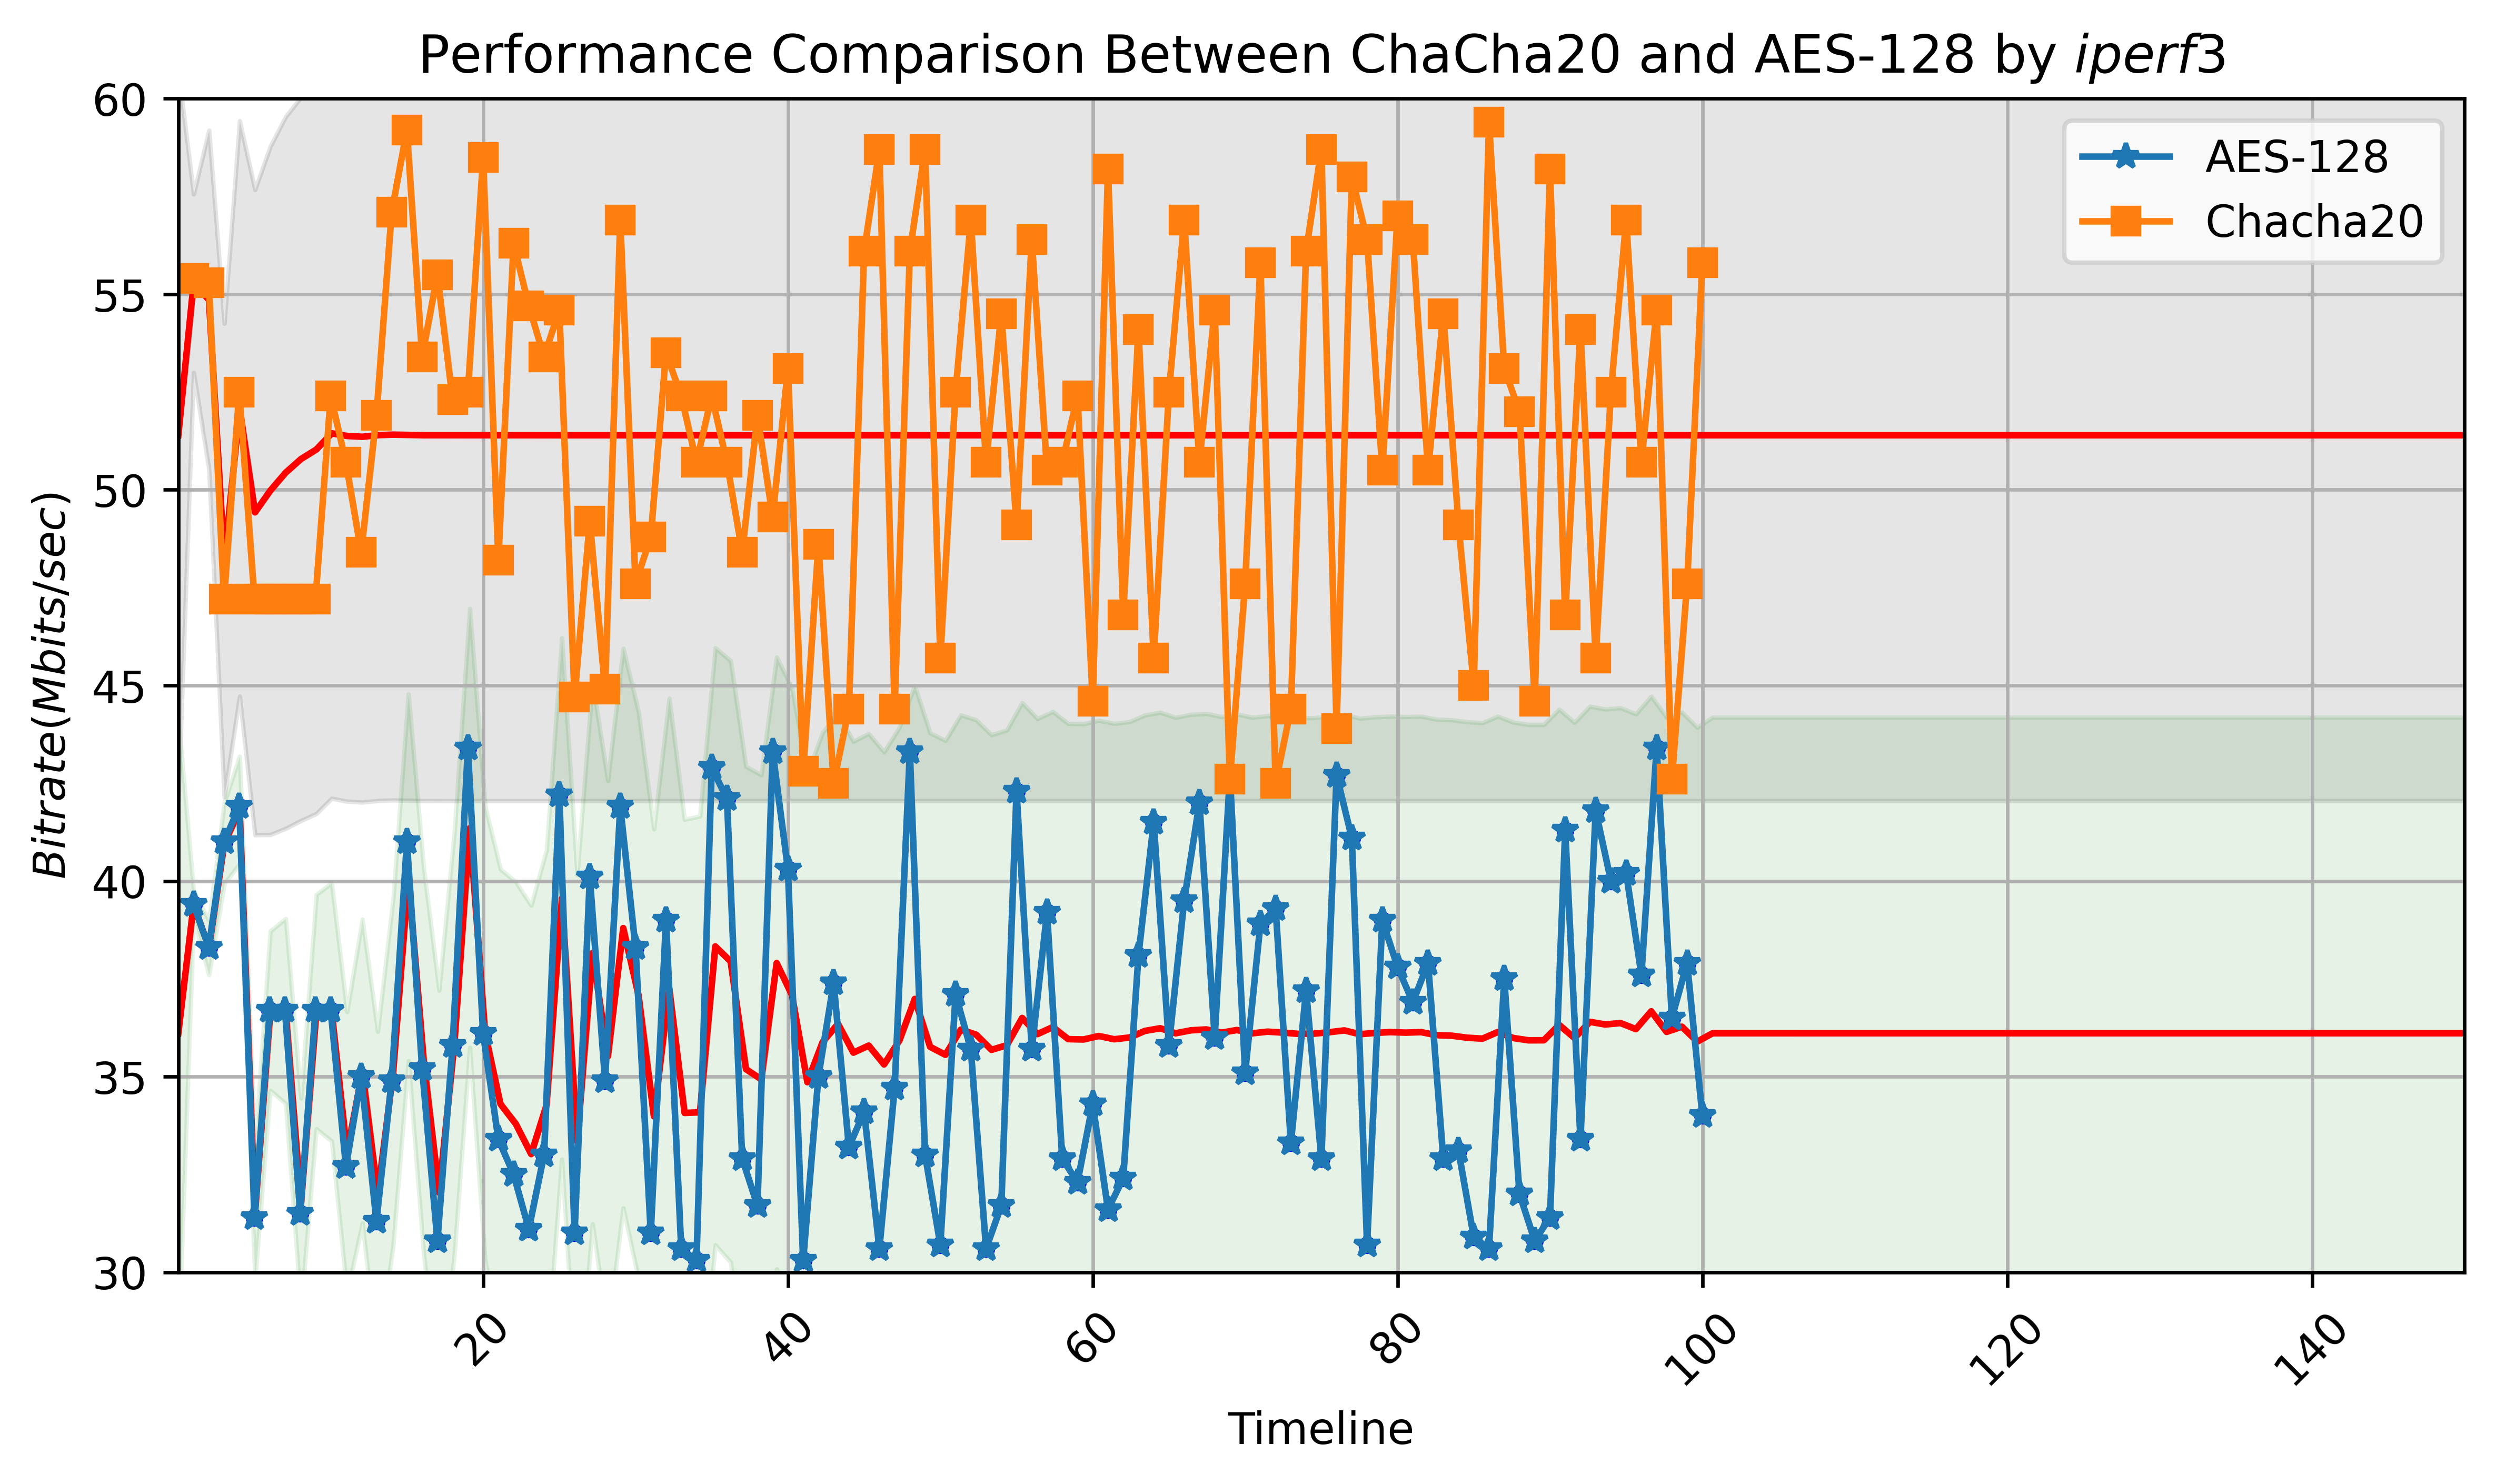
\includegraphics[width=0.67\linewidth]{../figures/fig4-2.png}
    \caption{Performance Comparison Between ChaCha20 and AES-128}
    \label{fig:4-2}
\end{figure}
\end{frame}

%---------------------------------------------------------
\begin{frame}
  \frametitle{LoRa Node Implementation}
  The functionalities of LoRa nodes Alice and Bob by leveraging the Arduino programmable MCU board and IDE previously discussed.
  \begin{figure}
    \subcaptionbox{LoRa Node Implementation\label{LoraNodeImplate}}
    {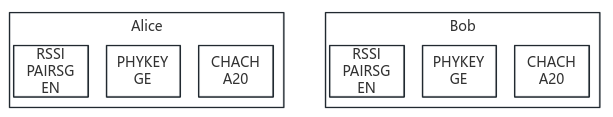
\includegraphics[width=0.7\linewidth]{../figures/LoraImplate.png}}
    \subcaptionbox{LoRa Transmission Implementation\label{LoraTransimissionImplate}}
    {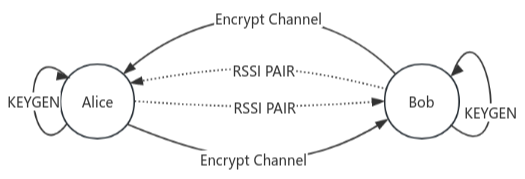
\includegraphics[width=0.6\linewidth]{../figures/LORAtransmit.png}}
    \caption{Implementation Details}\label{Implementation Details}
  \end{figure}
\end{frame}

\begin{frame}
  \frametitle{Test Implementation}
  As shown in Figure, in Liangkou Town, Conghua District, Guangzhou City. a sampling point (Bob) deployed on a tower for monitoring high-precision greenhouse gas flux. Alice(Temple) conducted an outdoor test from a temple located at a linear distance of around 300 meters from Bob.
  \begin{figure}
    \subcaptionbox{Conghua out door test\label{conghuatest}}
    {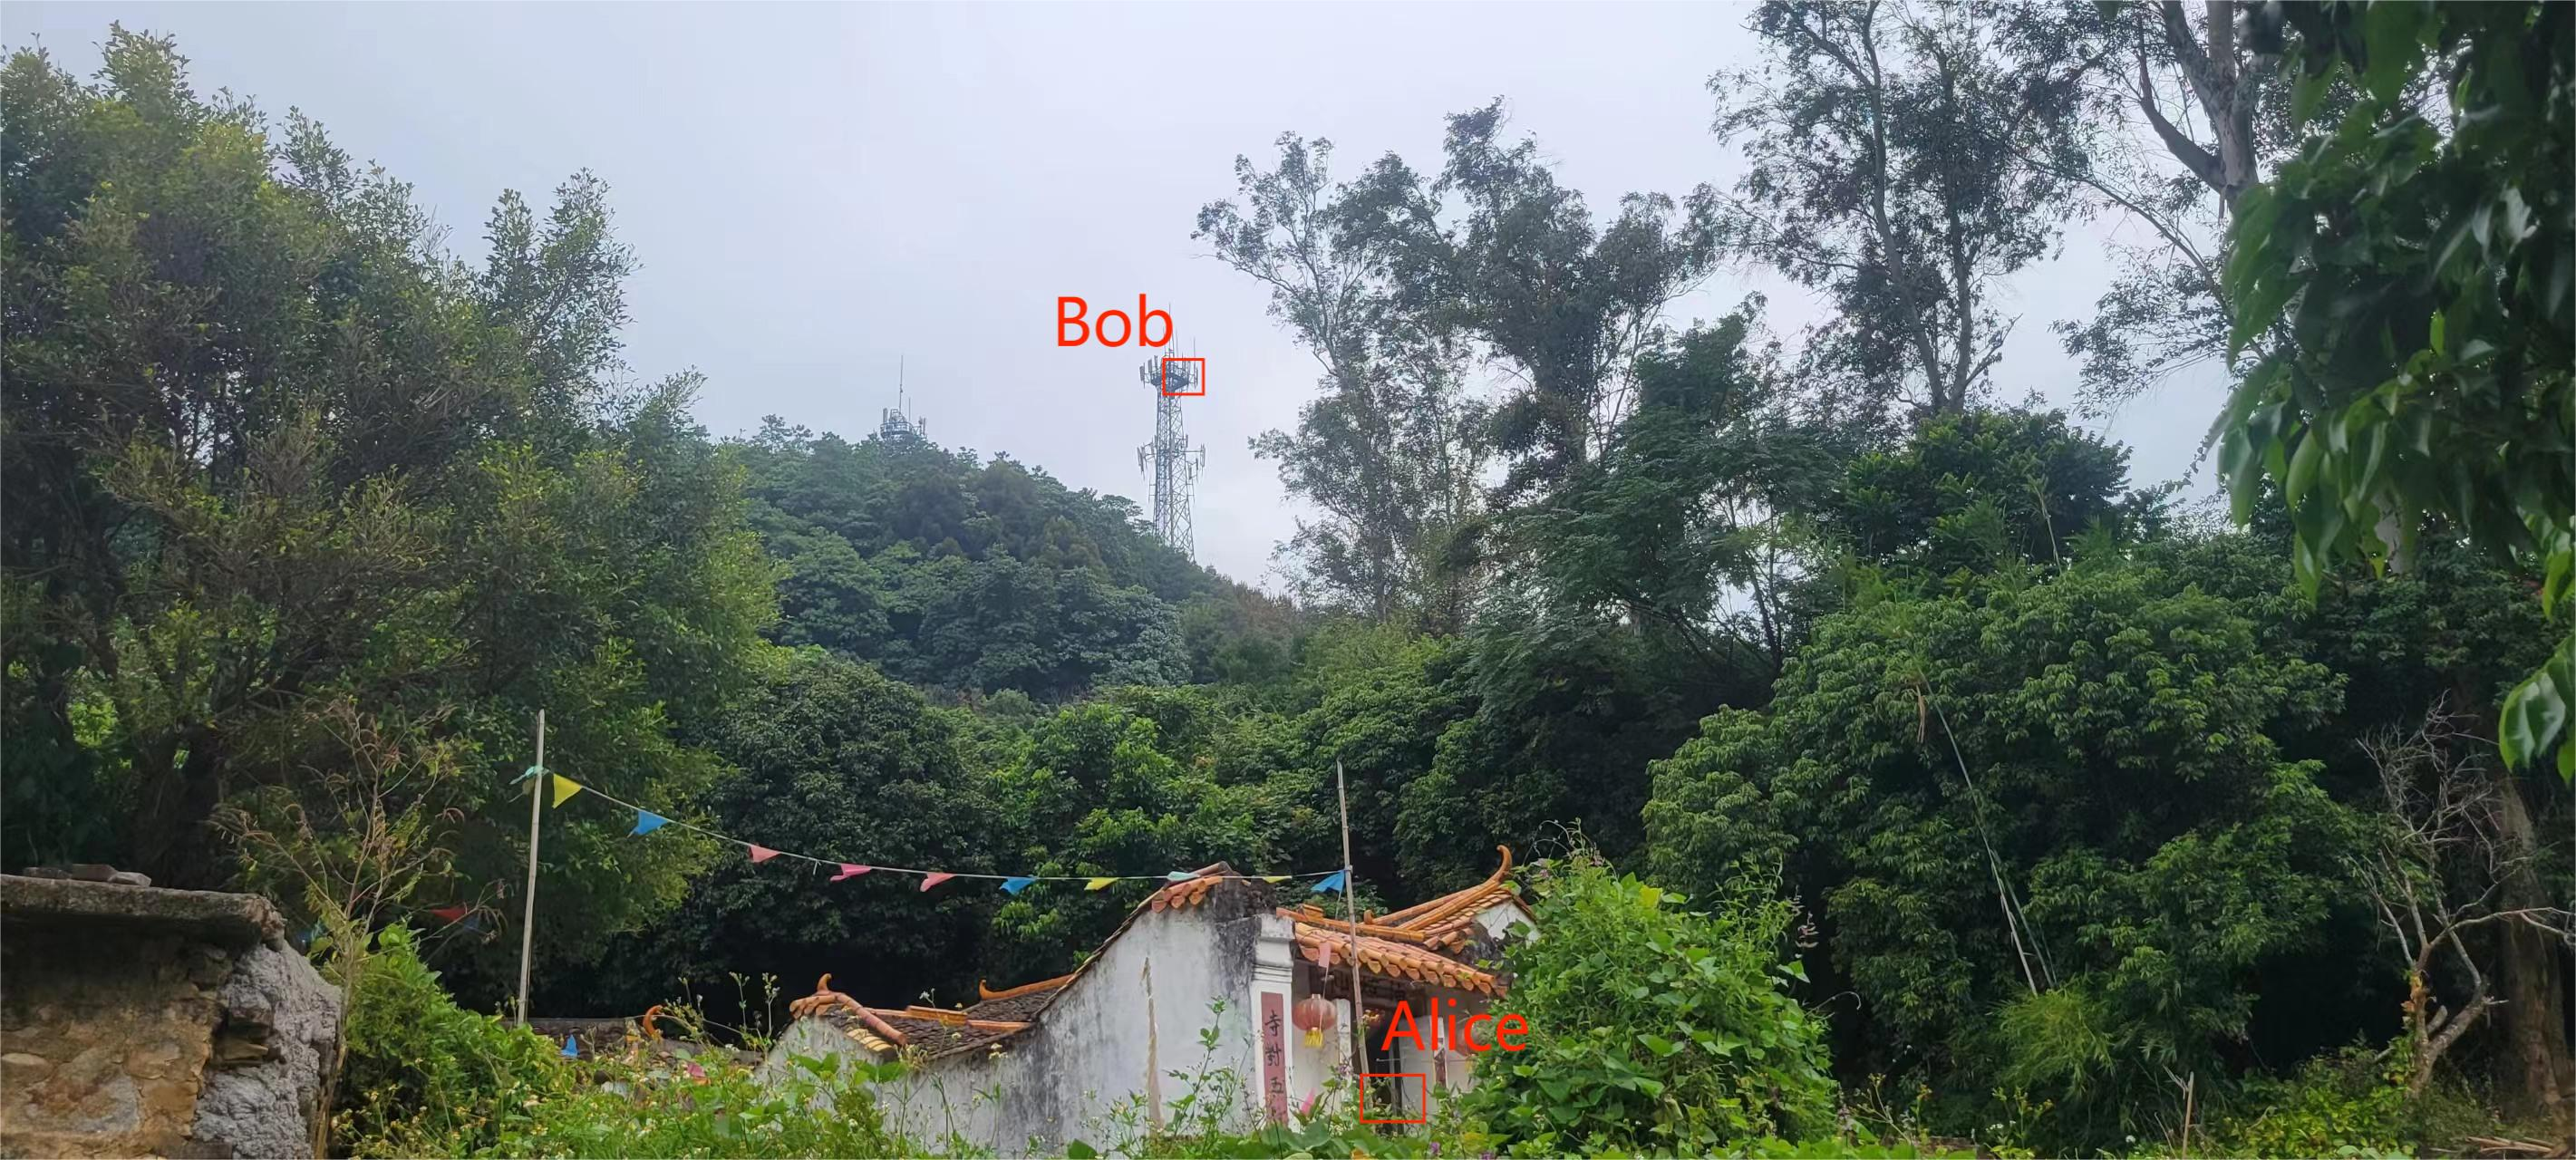
\includegraphics[width=0.72\linewidth]{../figures/conghua.jpg}}
    
    \caption{Deep-in-Building and Outdoor Test}\label{Test1}
  \end{figure}
\end{frame}

\begin{frame}
  \frametitle{Test Implementation}
  Figure represents an outdoor test conducted at the central area of Guangzhou Higher Education Mega Center.And involving high-power instruments and electromagnetic field interference.
  
  \begin{figure}
    \subcaptionbox{Panyu out door test\label{panyutest}}
    {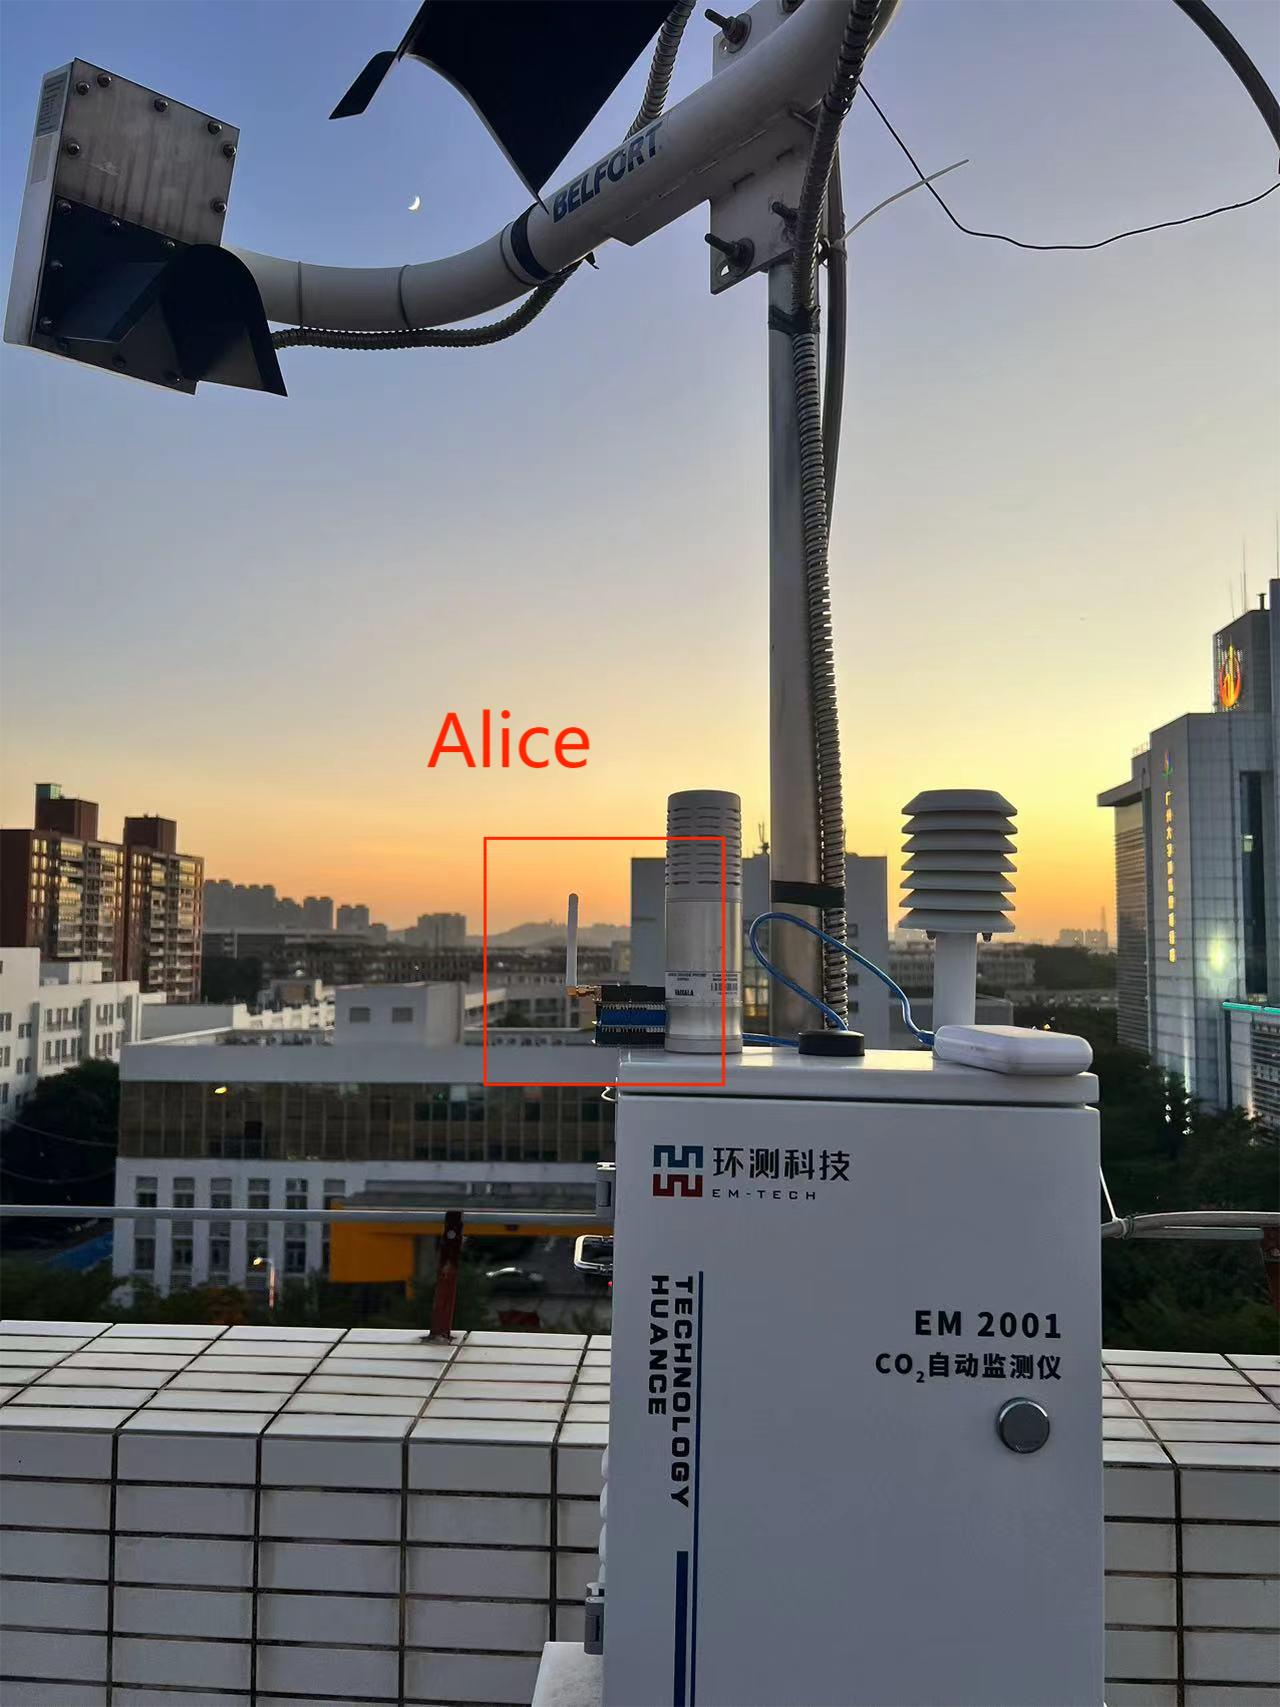
\includegraphics[width=0.25\linewidth]{../figures/panyuhighereducationmegacenter.jpg}}
    \subcaptionbox{Near instruments test\label{neartheinstruments}}
    {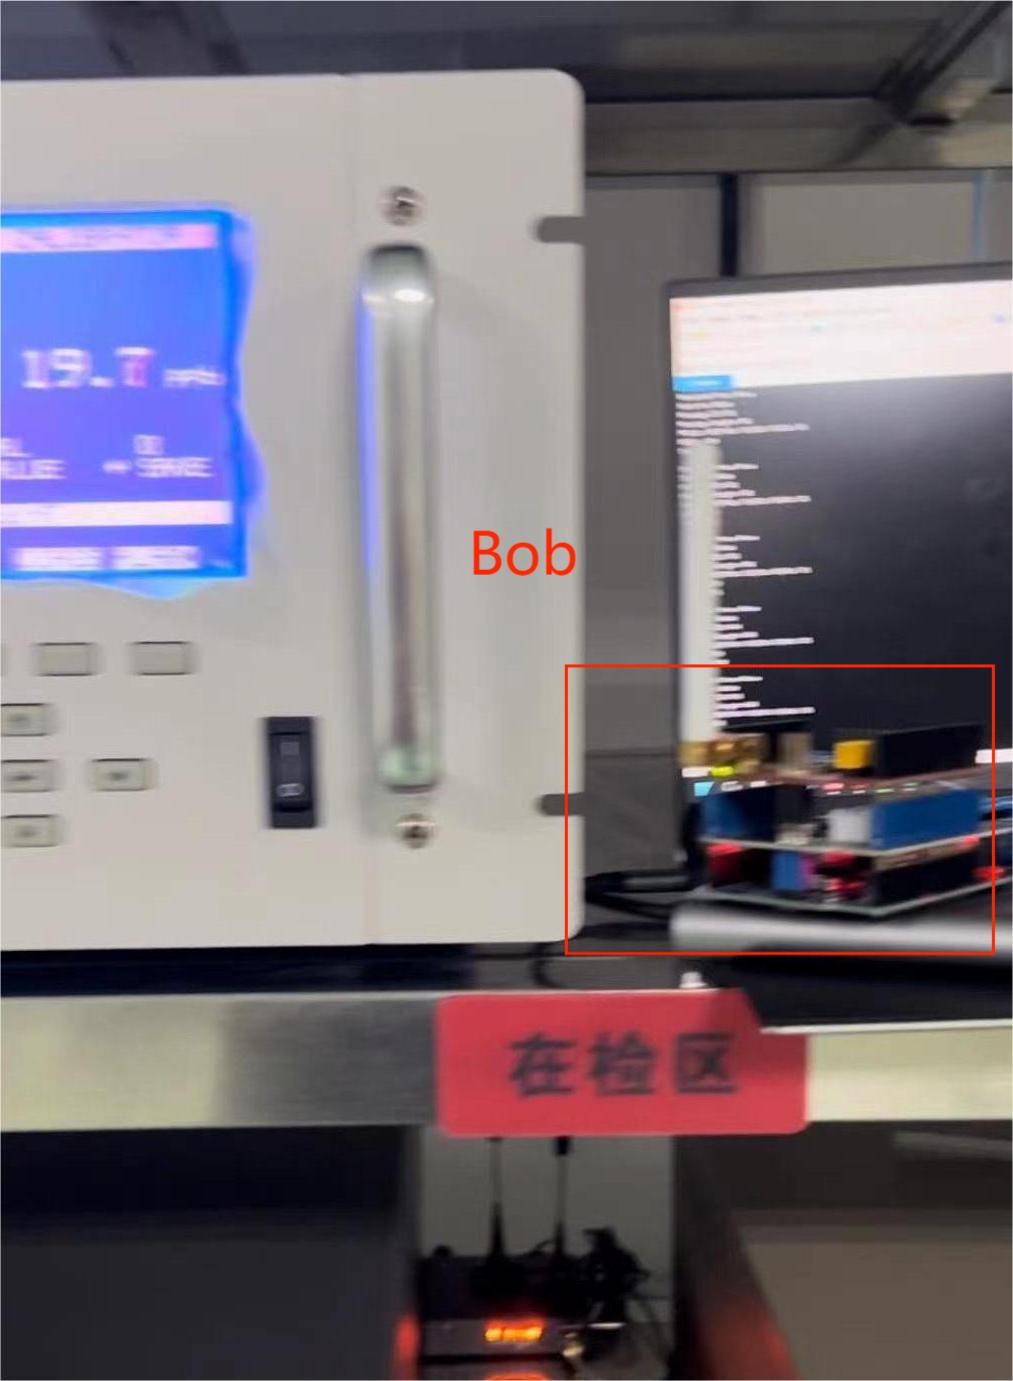
\includegraphics[width=0.246\linewidth]{../figures/neartheinstruments.jpg}}
    \subcaptionbox{In building test\label{inbuildingtest}}
    {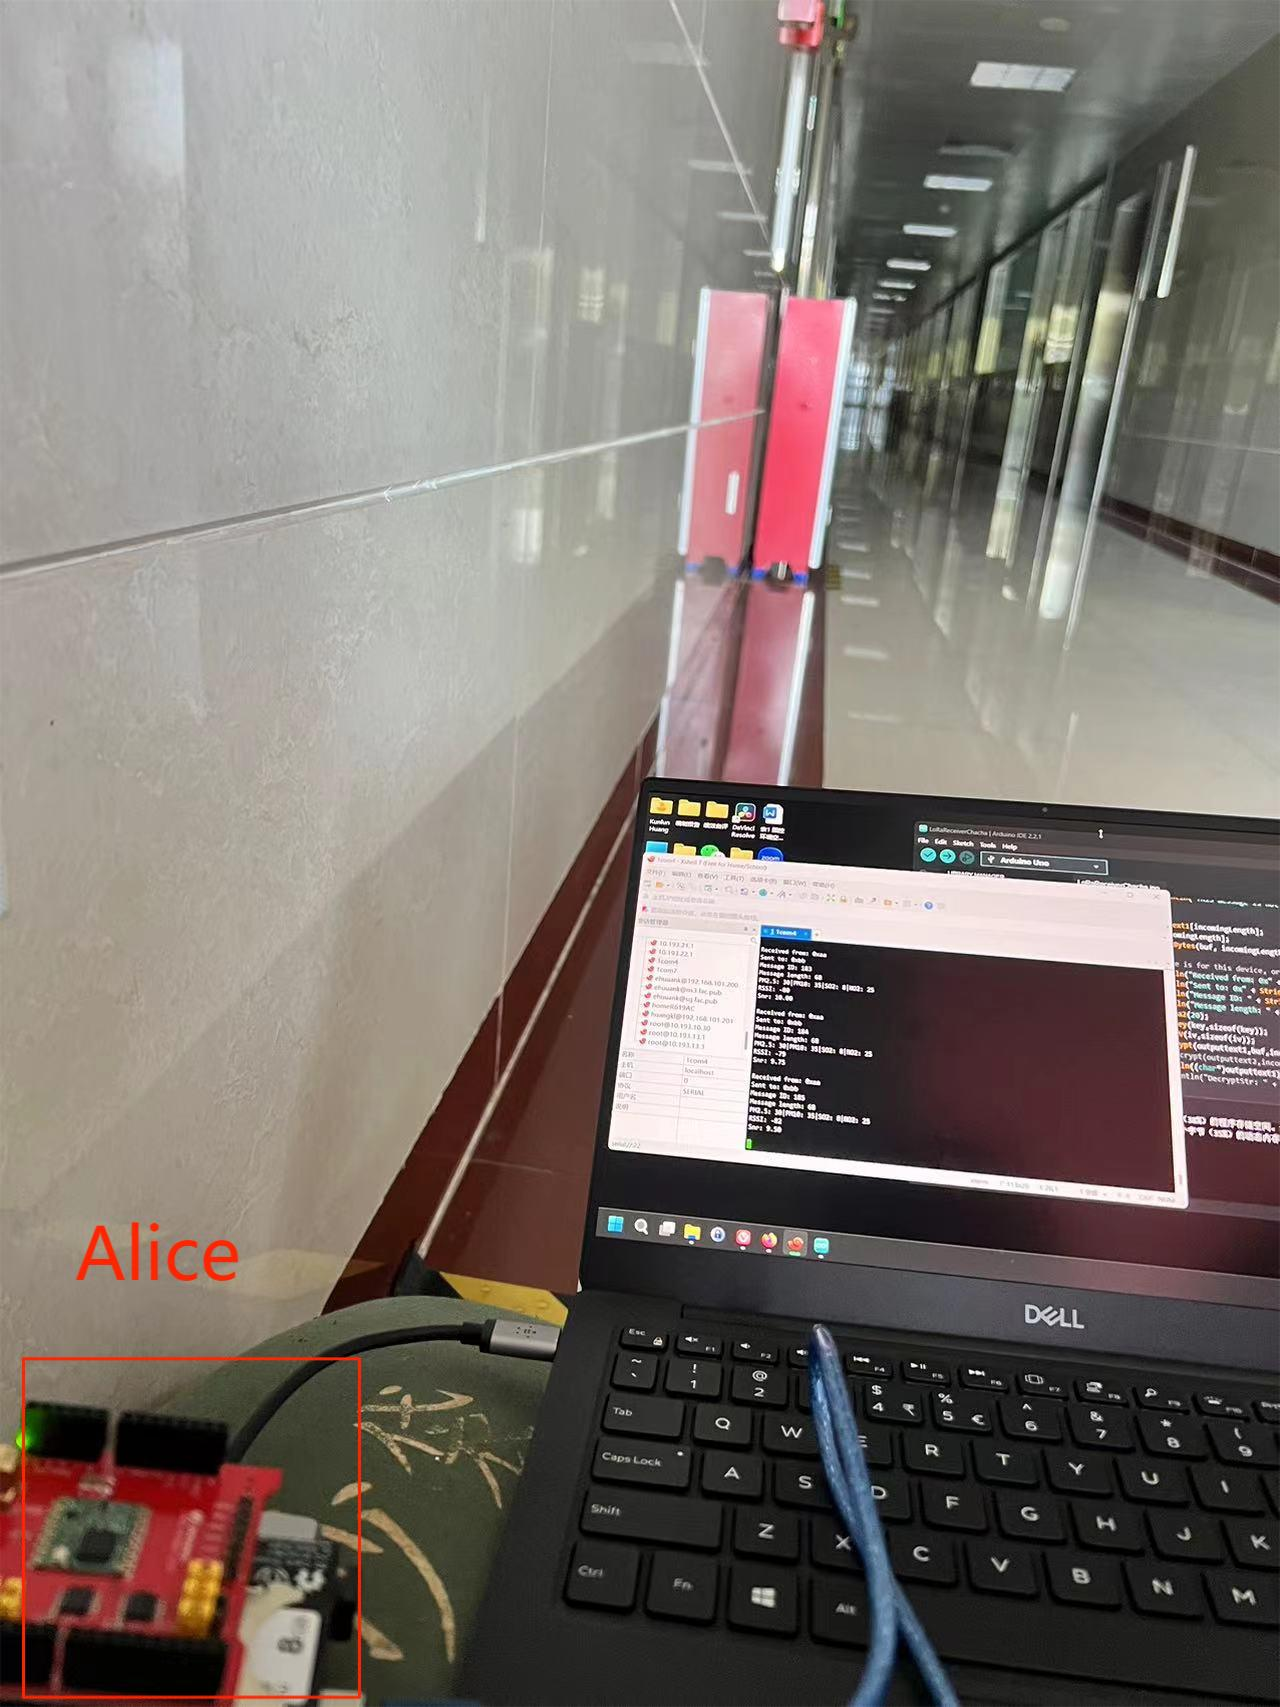
\includegraphics[width=0.25\linewidth]{../figures/inbuildingtest.jpg}}
    \caption{Deep-in-Building and Outdoor Test}\label{Test2}
  \end{figure}
\end{frame}

\begin{frame}
  \frametitle{RSSI Pairs Generation}
  Through the aforementioned tests, our LoRa nodes utilized a half-duplex-based protocol for exchanging RSSI pairs. We collected a significant dataset, obtaining data in the form of \(n\) pairs \(\underbrace{\{RSSI_{Alice}^1, RSSI_{Bob}^1\}...\{RSSI_{Alice}^n, RSSI_{Bob}^n\}}_{n\_pairs}\) through the serial port or Arduino's storage card. Figure shows the serial port displaying the sampling in LoRa Node.
\begin{figure}
  \centering
  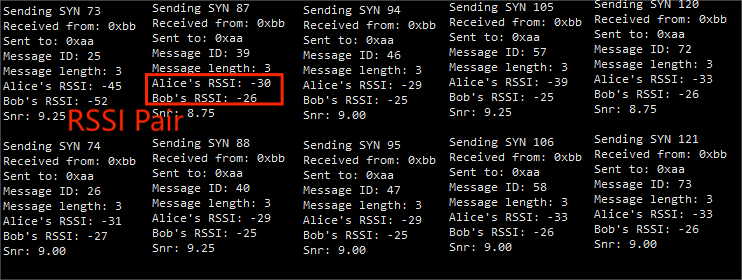
\includegraphics[width=0.67\linewidth]{../figures/sampling5.png}
  \caption{Sampling in LoRa Node}
  \label{sampling5}
\end{figure}
\end{frame}

\begin{frame}
  \frametitle{Key Generation}
  Than a program that implemented constitutes a crucial section of the thesis, focusing on LoRa physical layer key generation.
  \begin{columns}
    \column{0.5\textwidth}
  \begin{figure}
    \centering
    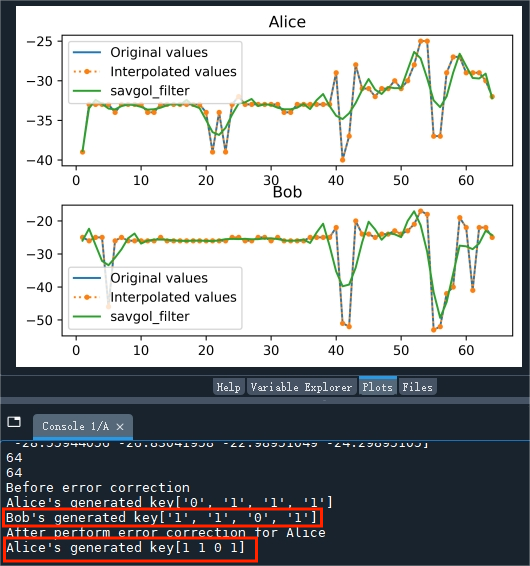
\includegraphics[width=0.82\linewidth]{../figures/physicalkeygen.png}
    \caption{Result of Performing Key Generation}
    \label{physicalkeygen}
  \end{figure}
  \column{0.5\textwidth}
  \begin{block}{Remark} 
    Prior to error correction, the bit keys they generated were not identical. After Alice applied error correction, they successfully obtained the same key.
    [ 1 1 0 1 ] 
  \end{block}
  
\end{columns}
\end{frame}


\begin{frame}
  \frametitle{Key Generation}
  After the key has been generated, it can be utilized in conjunction with encryption algorithms to secure data for transmission. Alice sends emulated environmental monitoring data to Bob.

  \begin{figure}
    \centering
    \subcaptionbox{Alice\label{Alice}}
    {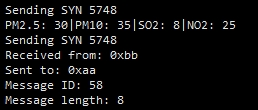
\includegraphics[width=0.38\linewidth]{../figures/chachaalice.png}}
    \subcaptionbox{Bob\label{Bob}}
    {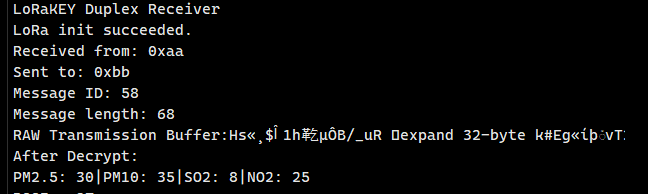
\includegraphics[width=0.6\linewidth]{../figures/chachabob.png}}
    \caption{Data Encrypt and Decrypt between Alice and Bob}\label{Data Encrypt and Decrypt}
  \end{figure}
\end{frame}

\begin{frame}
  \frametitle{Performance Analysis - Sampling Data Analysis}

  \begin{figure}
    \centering
    \subcaptionbox{LR - Conghua\label{conghuaanalystlr}}
    {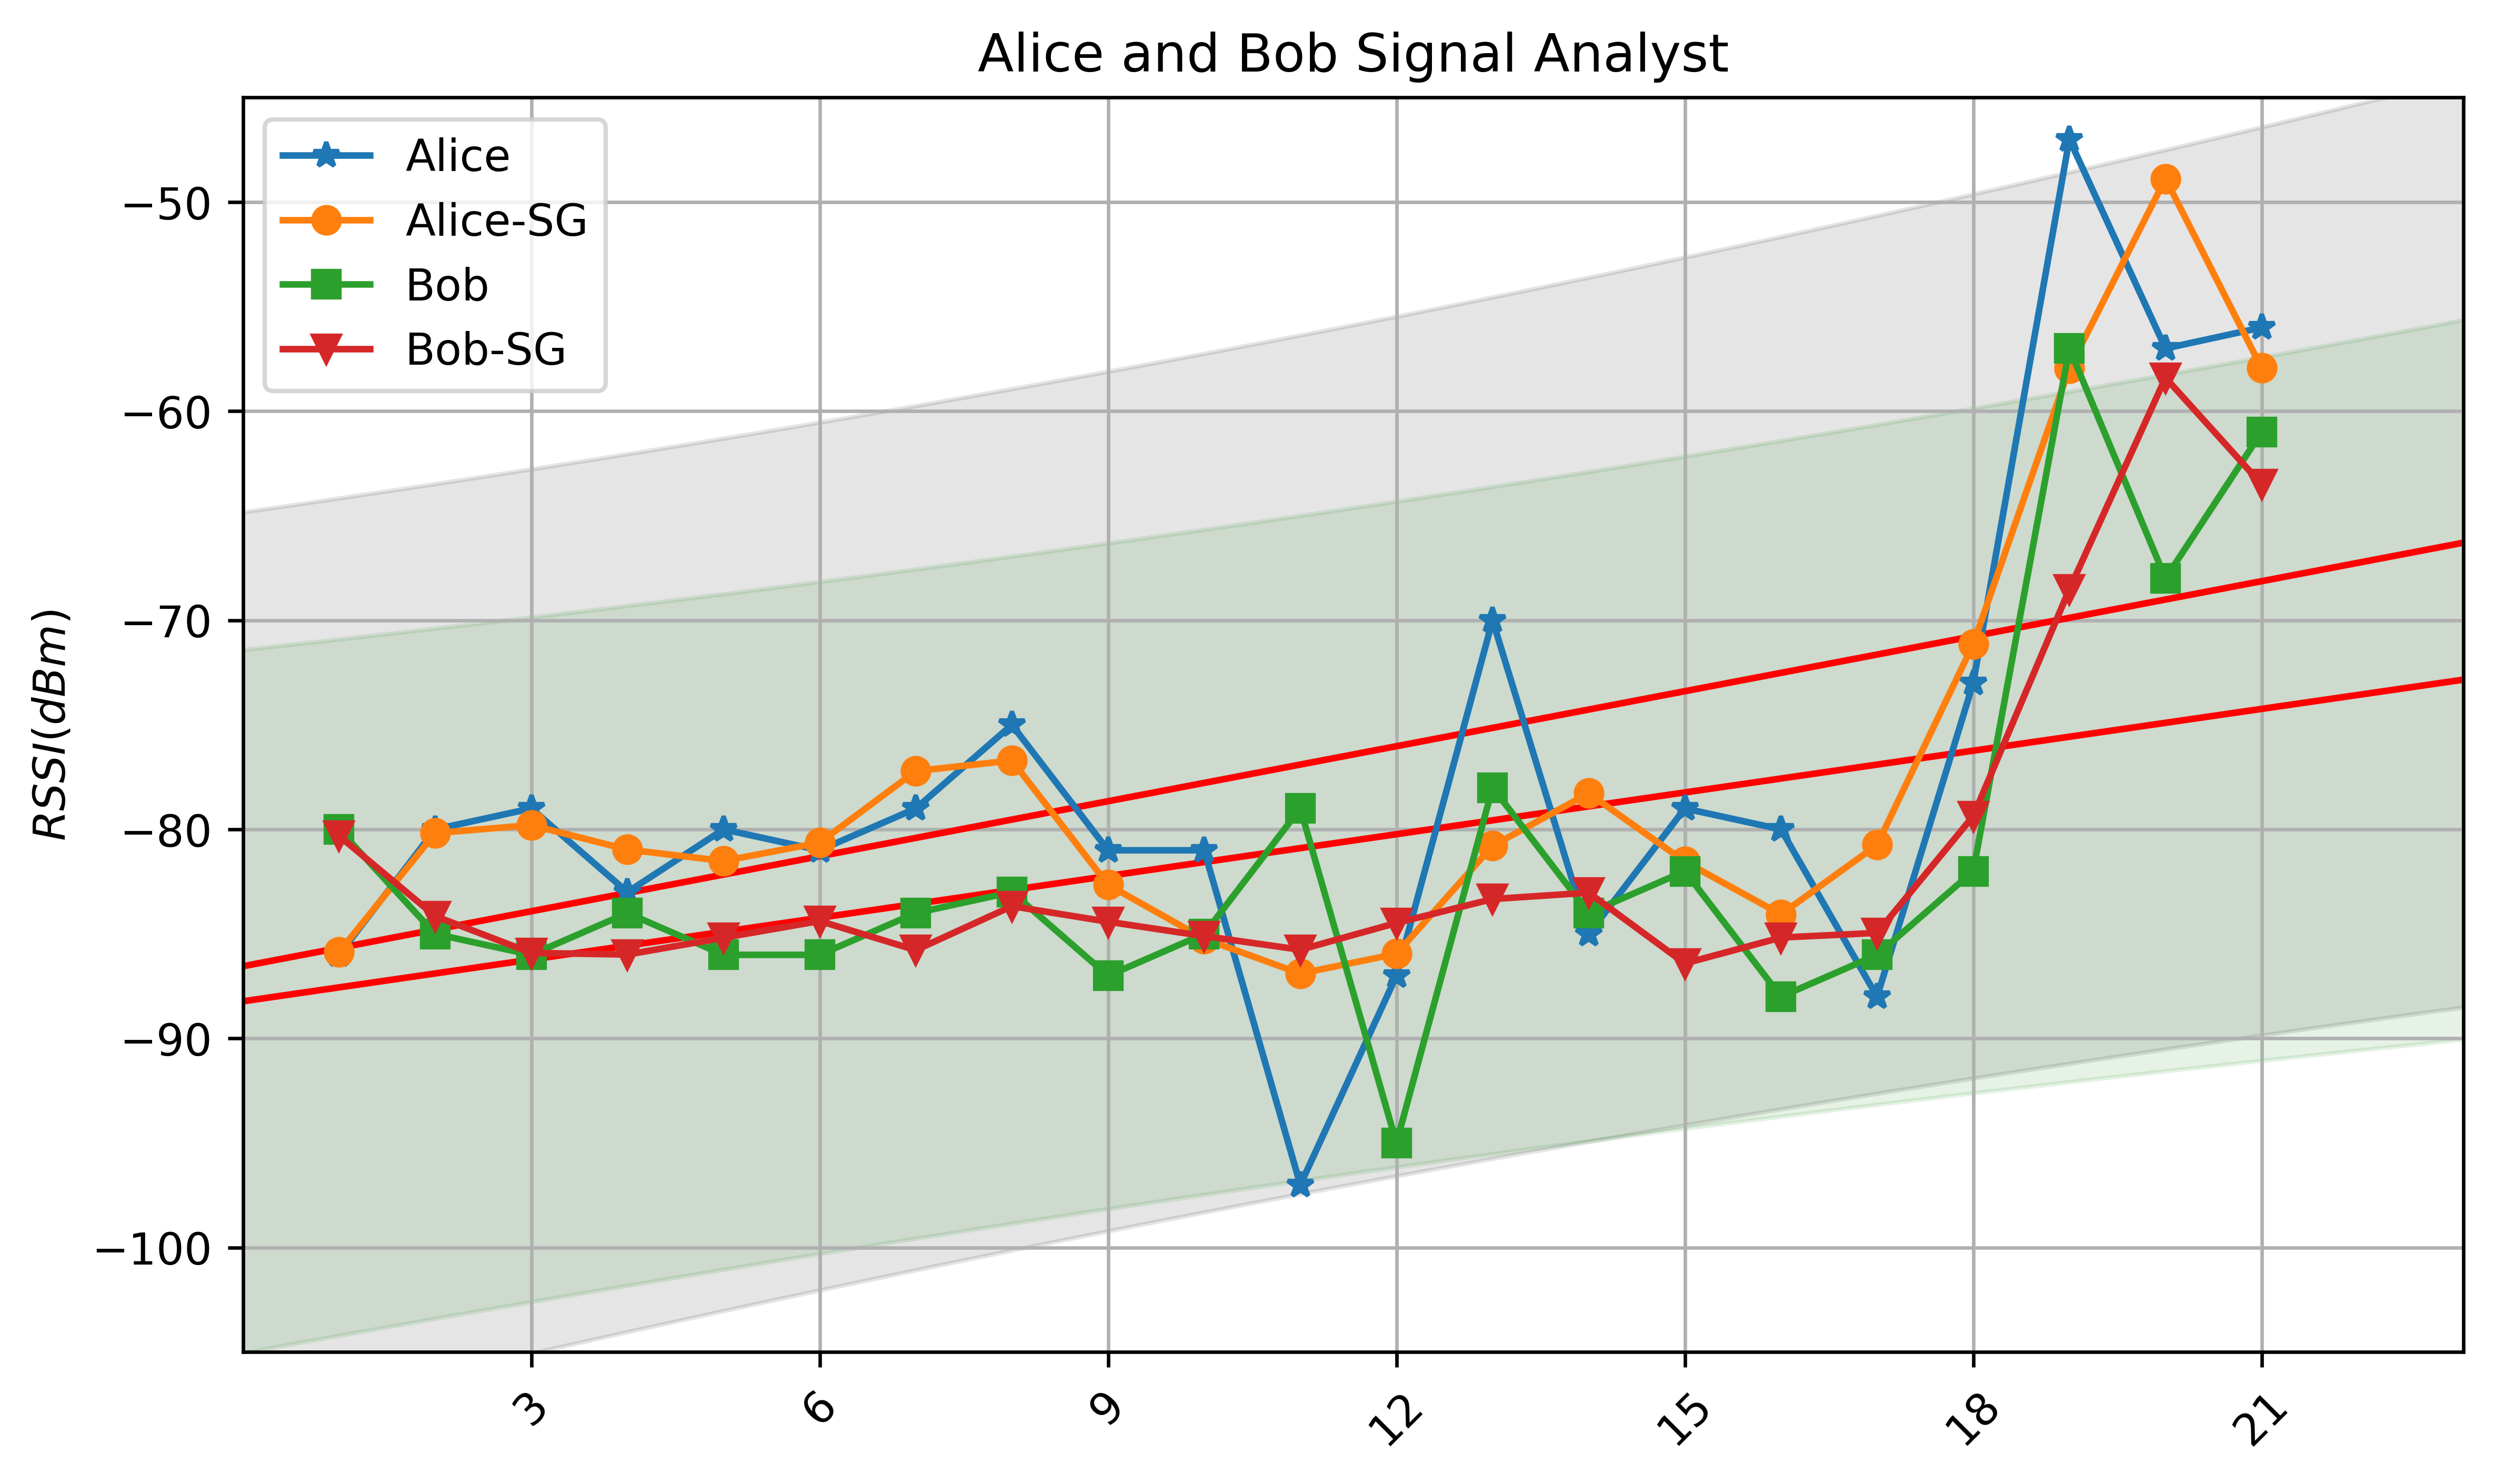
\includegraphics[width=0.421\linewidth]{../figures/conghuaanalystlr.png}}
    \subcaptionbox{RBF - Conghua\label{conghuaanalystrbf}}
    {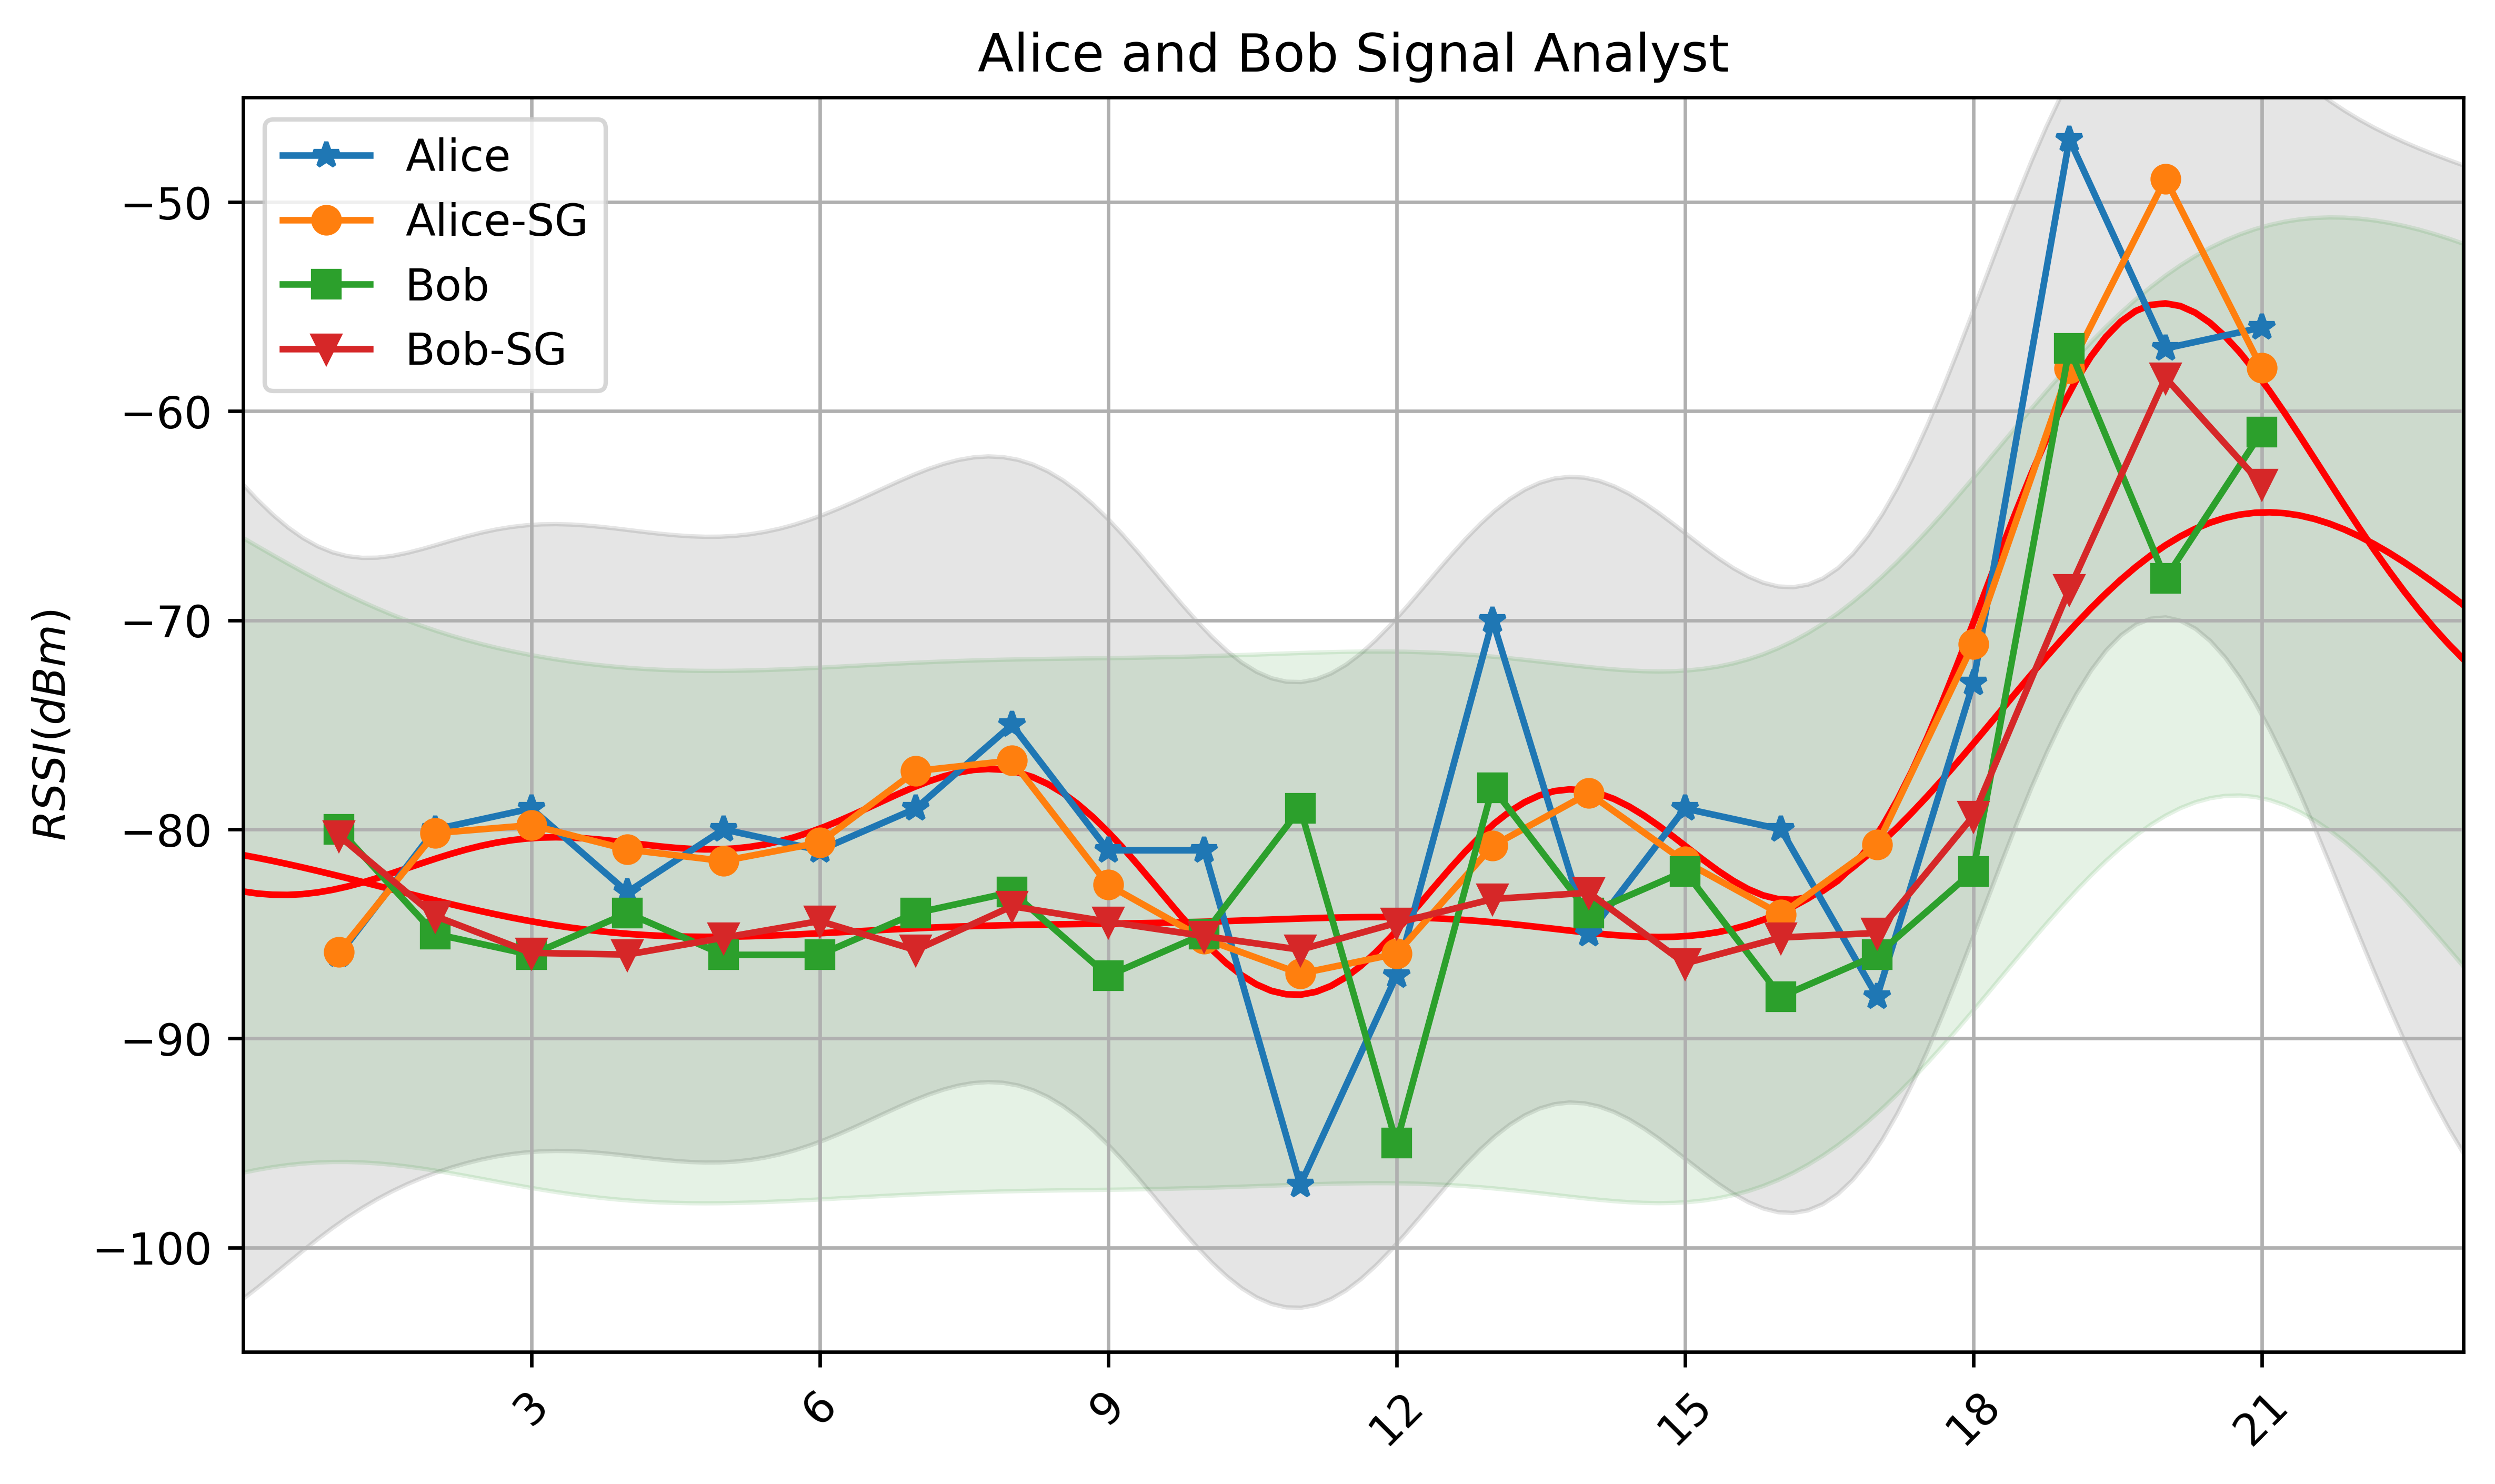
\includegraphics[width=0.421\linewidth]{../figures/conghuaanalystrbf.png}}
    \subcaptionbox{LR - Near Instruments\label{neartestanalystlr}}
    {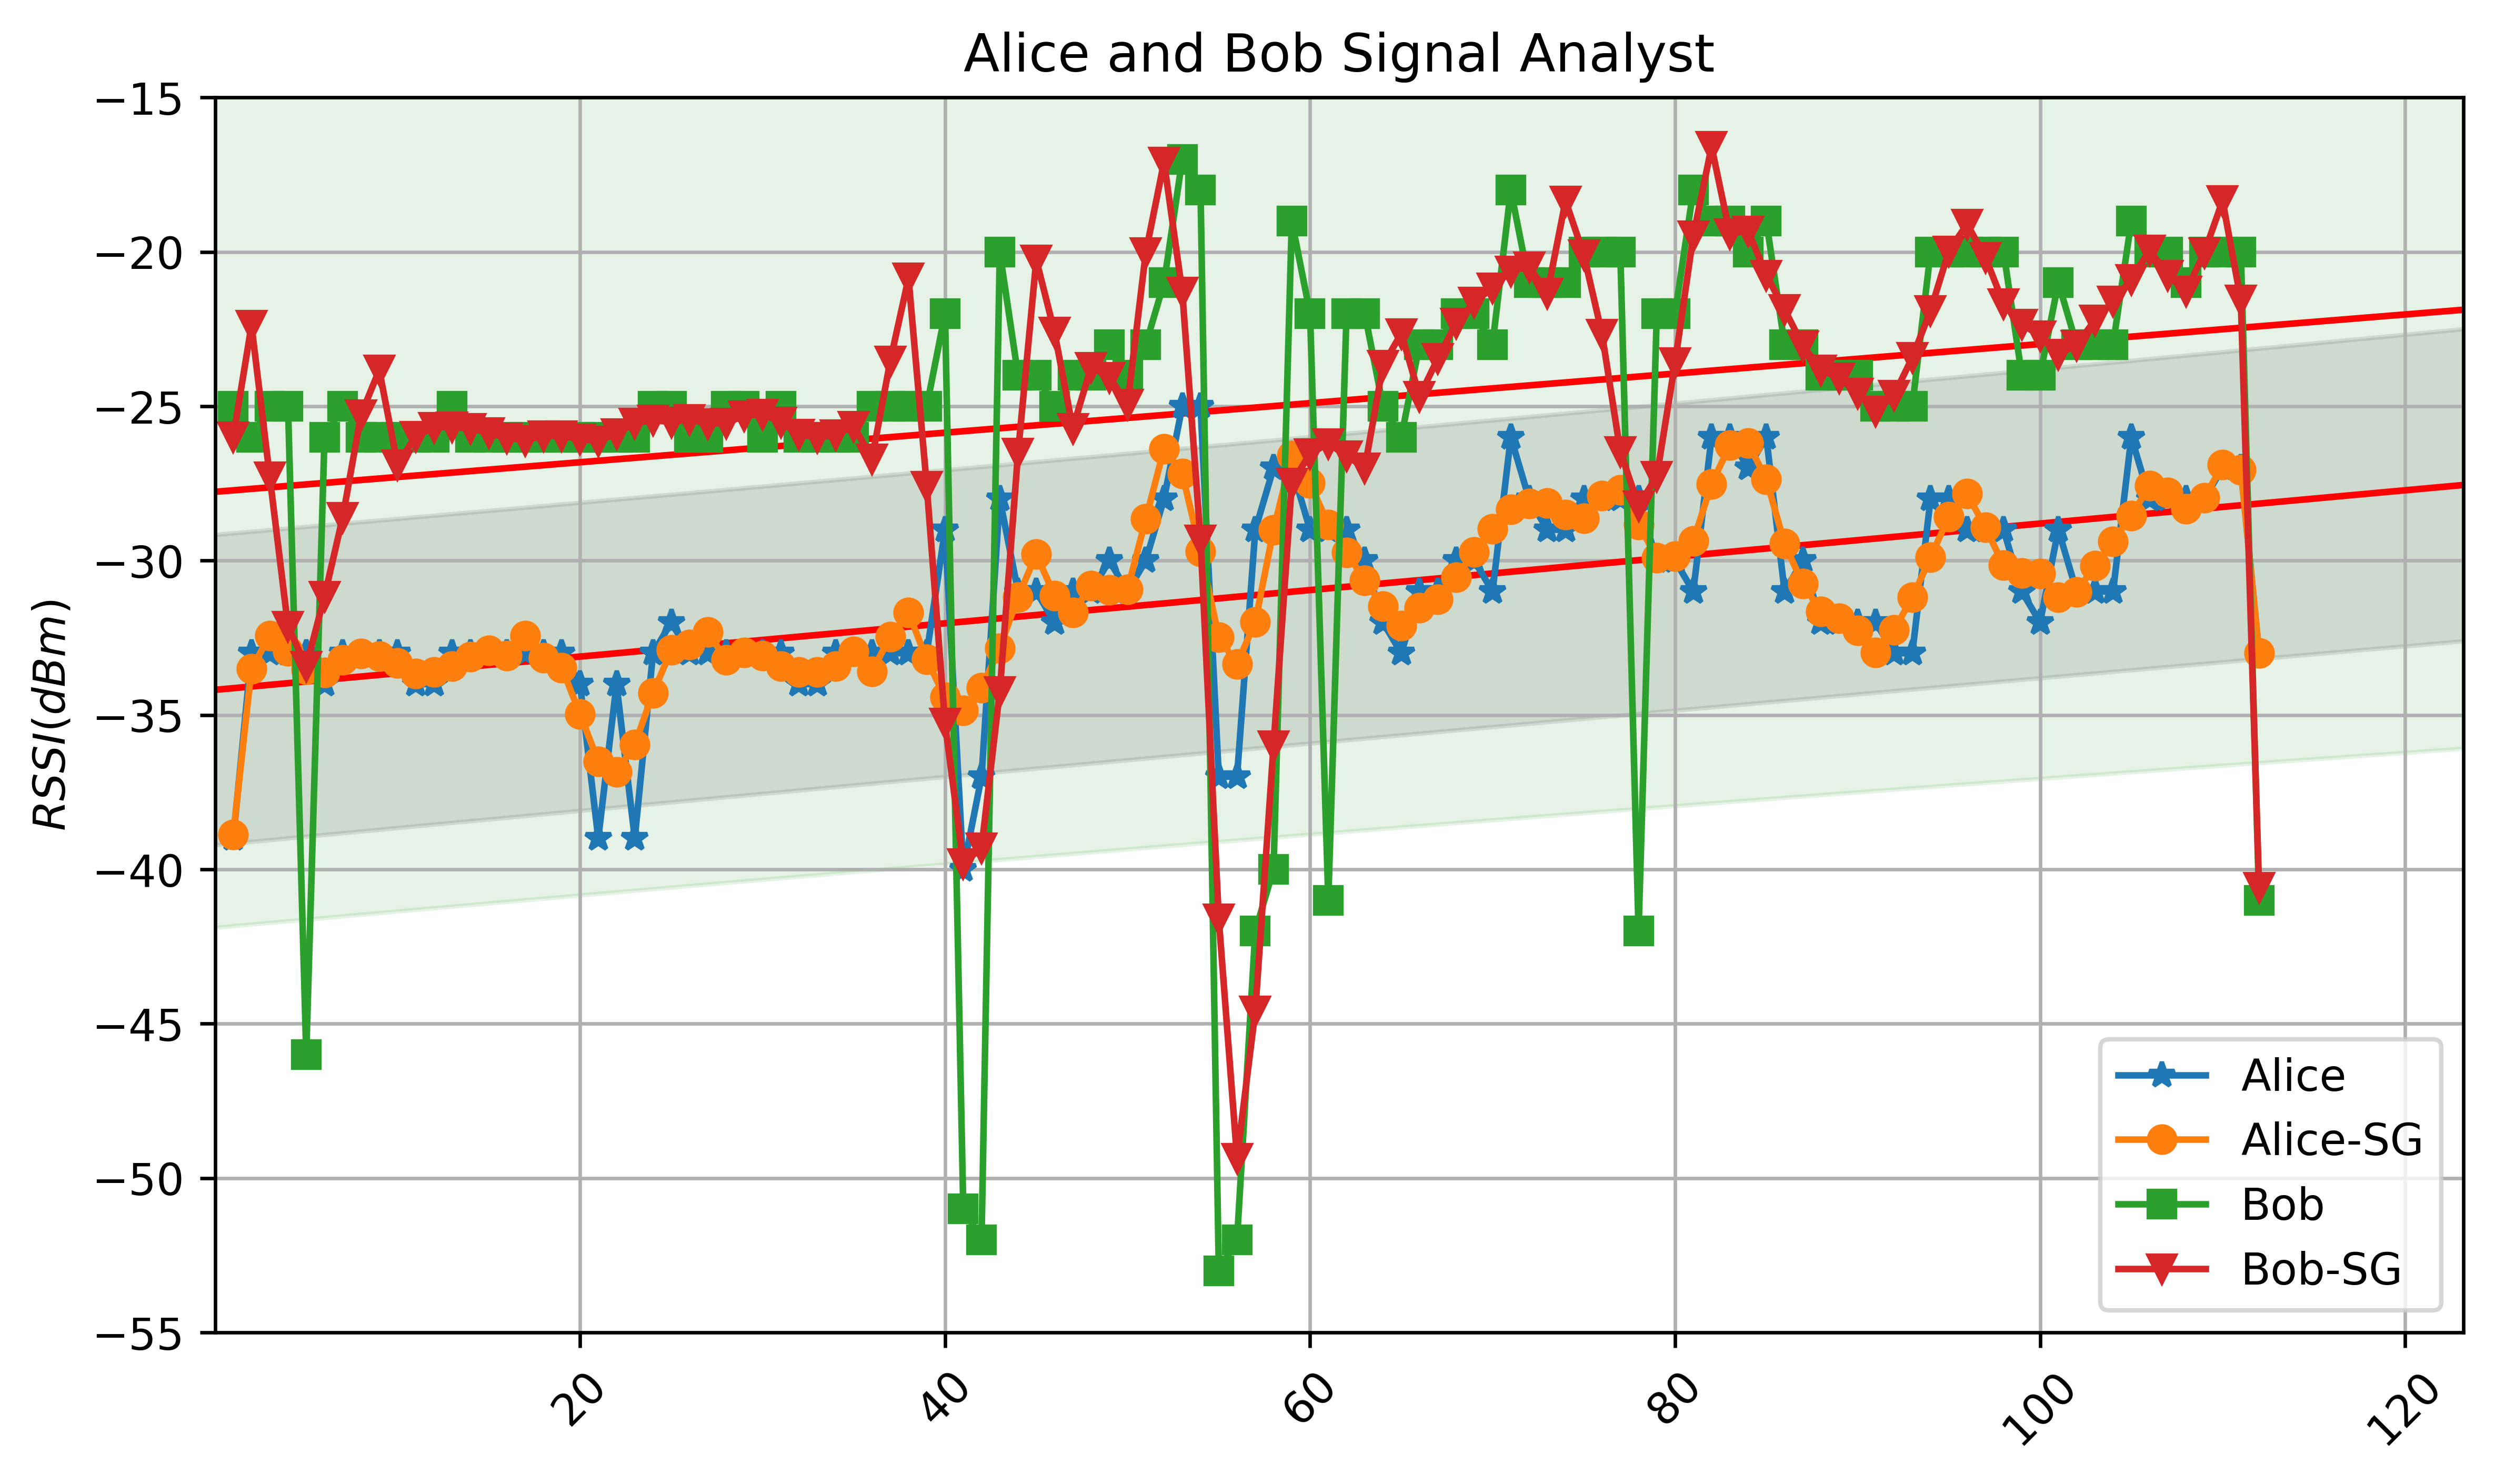
\includegraphics[width=0.421\linewidth]{../figures/neartestanalystlr.png}}
    \subcaptionbox{RBF - Near Instruments\label{neartestanalystrbf}}
    {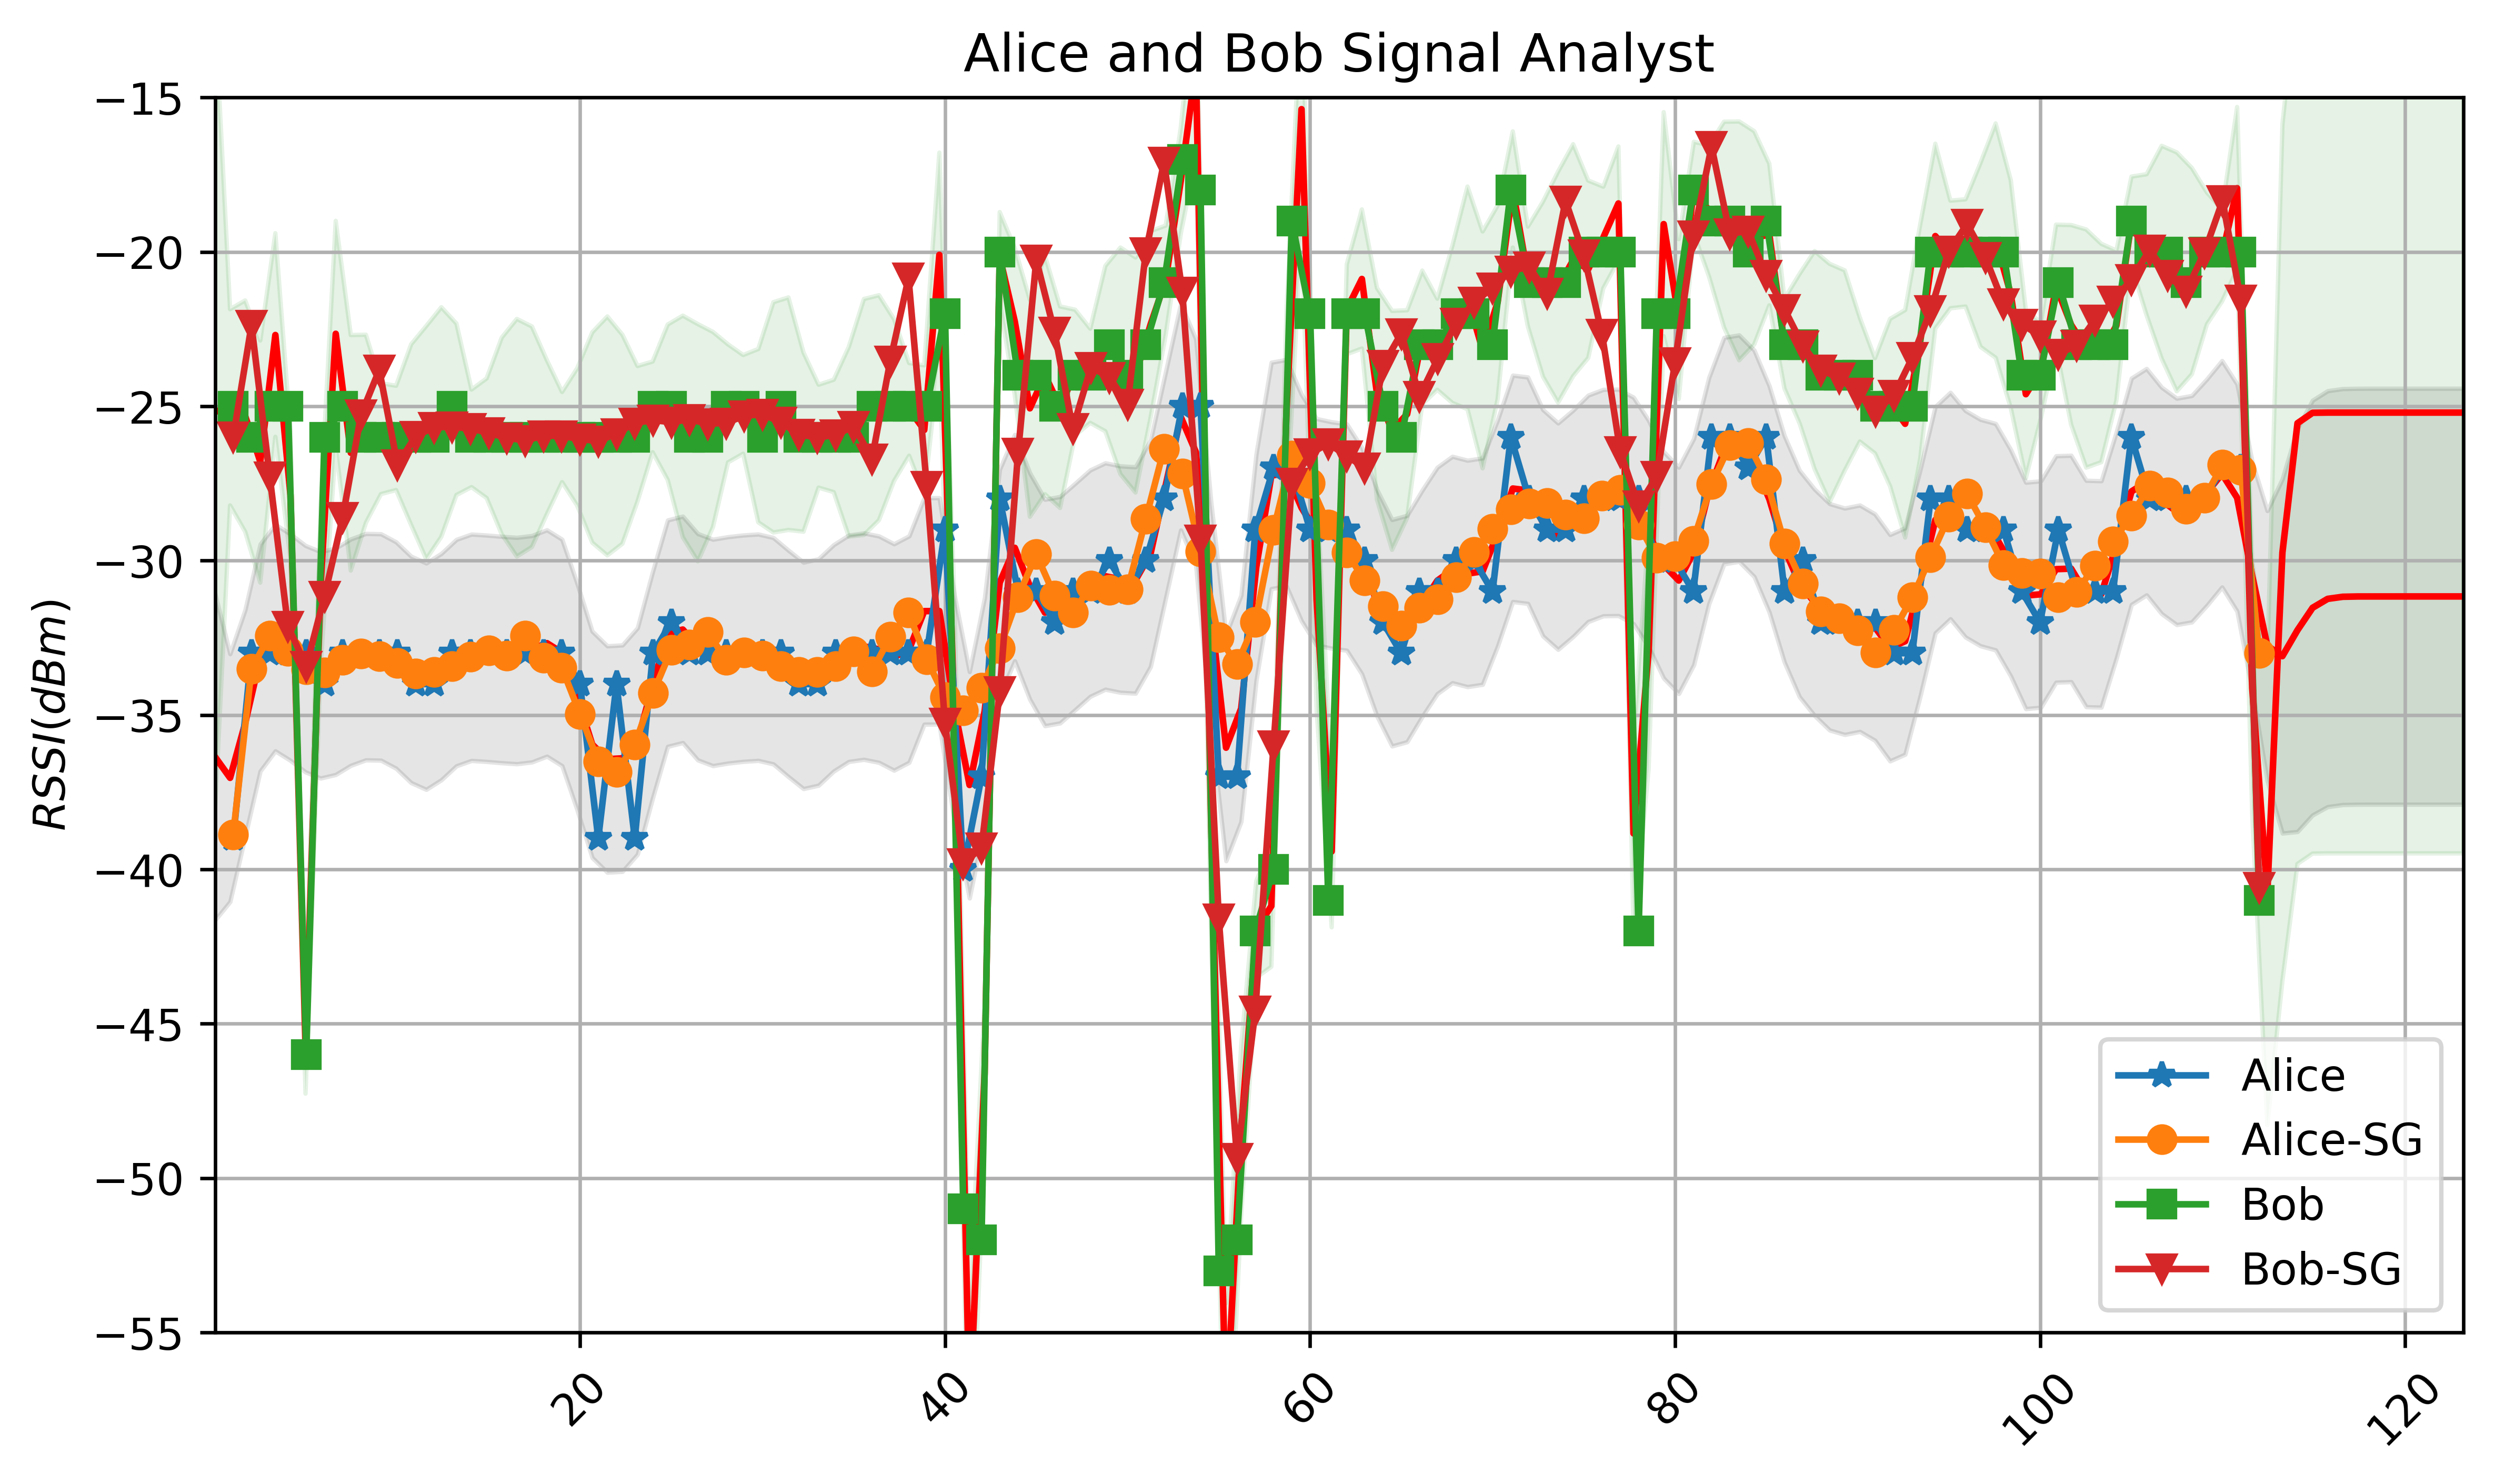
\includegraphics[width=0.421\linewidth]{../figures/neartestanalystrbf.png}}
    \label{Sampling Data Analysis}
  \end{figure}
\end{frame}

\begin{frame}
  \frametitle{Performance Analysis -  Key Generation Analysis}

  The performance of physical layer key generation by using LoRa-Key under varying parameters are analyzed in this part.
  \begin{figure}
    \centering
    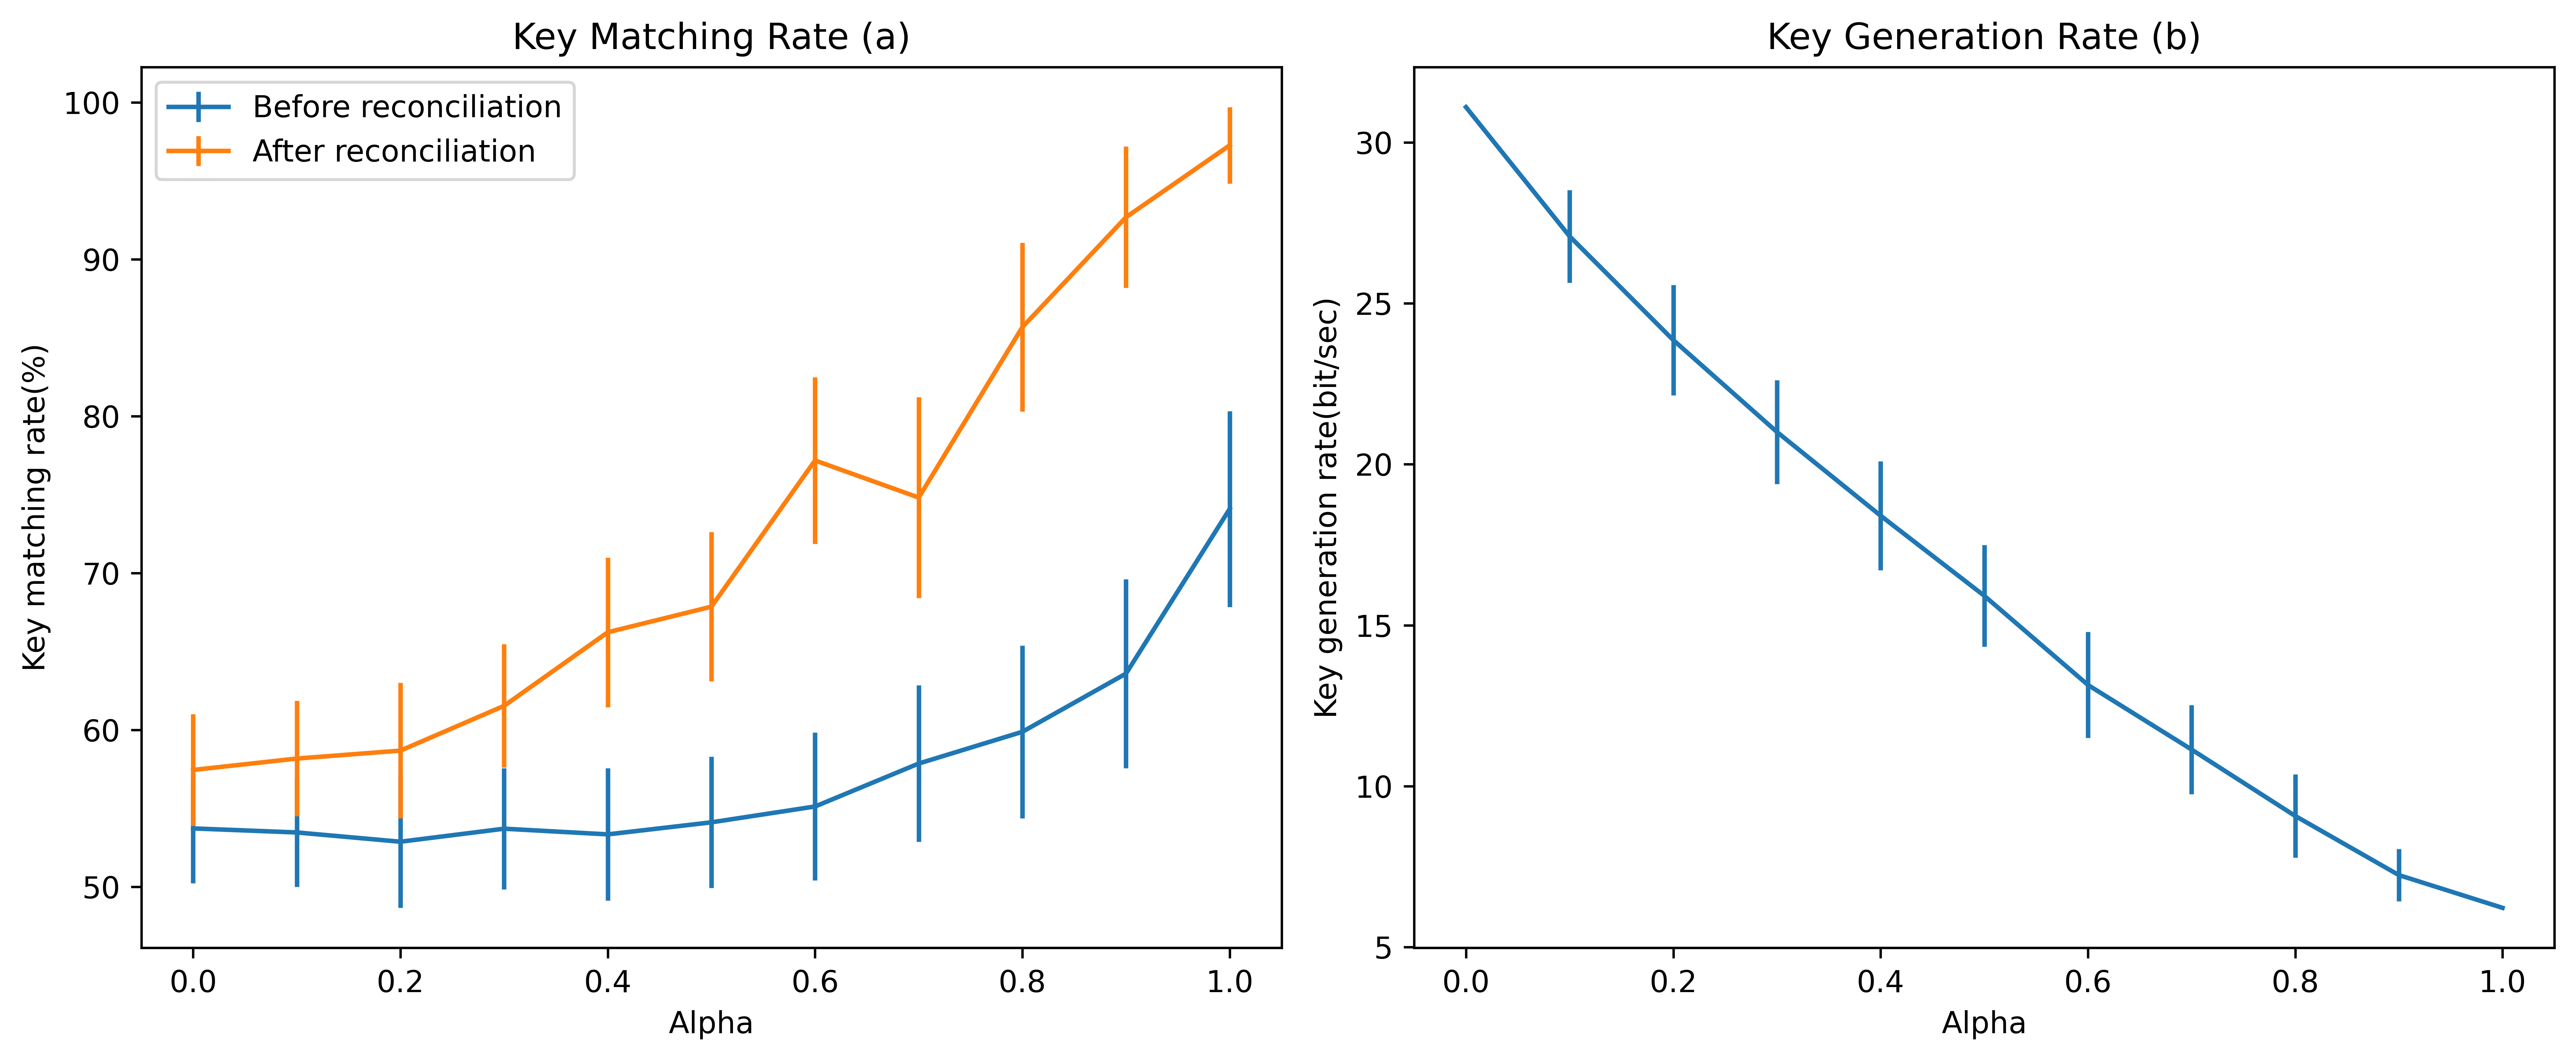
\includegraphics[width=0.8\linewidth]{../figures/keygenanalyst.png}
    \caption{Key Generation Analysis}
    \label{keygenanalyst}
  \end{figure}
A noticeable improvement in the bit agreement rate is observed after the implementation of the reconciliation technique, with the key agreement rate reaching 100$\%$ when \(\alpha\) rises to 1. 

\end{frame}
%---------------------------------------------------------

\section{Conclusion}

%---------------------------------------------------------
%Example of the \pause command
\begin{frame}
  \frametitle{Conclusion}
  The study has specifically explored methods and algorithms for physical layer key generation in wireless communication, with a spotlight on the LoRa protocol. The implementation of LoRa nodes, a RSSI-based physical key generation, a Chacha20 encryption in LoRa nodes, and various signal processing techniques has been presented, along with real-world tests in both outdoor and indoor environments.
\vspace{0.2in}
  \begin{itemize}
    \item IoT and WSNs Study
    \item Physical Layer Key Generation Study and Implementation
    \item Intersection of computer disciplines
    \item Project Management \footnotemark
    \item Self-motivated Improment
    \end{itemize}
\footnotetext[1]{PM by Git: https://github.com/hiplon/CityUCS6534GuideStudy}
\end{frame}
%---------------------------------------------------------

\appendix
\begin{frame}
  \frametitle{Acknowledgement}
  This Guide Study was greatly helped by Prof. Xu, and many of the implementations were based on his research, and thanks to Ph.D. candidate Yang for providing Q\&A as well as help, and the equipment used for the study.
\end{frame}

\begin{frame}[allowframebreaks]{References} 
\fontsize{7pt}{7pt}\selectfont
\bibliographystyle{ieeetr} % 
\bibliography{refs} % Entries are in the refs.bib file
\end{frame}

\begin{frame}{Thanks} 
  \fontsize{23pt}{23pt}\selectfont
  \centering
  Thanks for your patience

  \vspace{0.2in}
  
  Q\&A
\end{frame}

\end{document}